\chapter{Improving Interactivity for Human-aware Intervention}
\label{chap:ch6}
Using the Rush Hour domain, we study how an intervention model can be extended to recover from intervention and help users complete cognitively engaging tasks by providing helpful hints. 
In the context of the Rush Hour puzzle solving task, a hint is a piece of information about the Rush Hour planning problem. 
We design helpful hints to allow the user to carefully probe the search space of the Rush Hour STRIPS planning task described in Section~\ref{sec:rushhourstrips} in
Chapter~\ref{chap:ch5} while avoiding the undesirable state.
Existing plan and goal recognition algorithms do not define a method for the user (or the software agent) to recover when the observer recognizes an undesirable state is developing and/or imminent.
In this chapter, we address that limitation by designing four helpful hints the observer presents to the user after intervening.
\begin{itemize}
\item The minimum remaining number of moves
\item The next best move
\item The vehicles that must be moved
\item Restart puzzle
\end{itemize}


In Chapter~\ref{chap:ch5}, we presented the Human-aware Intervention problem for the Rush Hour puzzle task as a tuple
$\mathcal{I} = (D, \desired, \undesired, \historyDef, \presentedAction, \mathcal{X}_\Diamond)$ be a tuple where
  $D=\langle F, A, \initialState \rangle$ is a planning domain,
  $\desired \subset F$ is a desirable state,
  $\undesired \subset F$ is an undesirable state,
  $\historyDef = ( o_1 [s_1], o_2 [s_2], \ldots, o_{i-1} [\historyEndState])$ is a history of previously observed actions and states, which started from \initialState with the implied resulting states in brackets.
  \presentedAction is the \emph{presented action} that the user would like to perform, and
  $\mathcal{X}_\Diamond = \emptyset$ because we can not use an automated planner to extract suffixes when a human user is solving the planning task.
The \textnormal{Intervention Problem} is a function $intervene (\mathcal{I}) :  \mathcal{I} \rightarrow \{No, Yes\} $
that determines for the presented action \presentedAction whether to intervene.
For Rush Hour, the observer relies on those implied states instead of just the actions to decide intervention.
Because we model the Rush Hour planning task as a deterministic state transition system,  it is easy to map between actions and states.

For the study discussed in this chapter, the observer uses the Rush Hour Human-aware Intervention model configured to use the lowest level of sensitivity (i.e., $k=1$).
When $k=1$, the observer predicts intervention one move before undesirable state occurs.
For each action the user executes, the observer solves the Human-aware Intervention problem $\mathcal{I}$ if the $intervene (\mathcal{I}) :  \mathcal{I} \rightarrow \{Yes\} $, the observer displays the hints to help the user decide what to do next.
We evaluate the effectiveness of the proposed intervention recovery approach with a human subject experiment.


\section{Motivation}
When a human user is learning to use a new software application, it can be helpful to have a passive observer that can intervene to help the user reach his intended goal. 
This is particularly important when using the software imposes a significant cognitive load on the user and as a result the user's plan to accomplish the intended goal can become vulnerable to unintended actions or events.
For this study, we simulate the human user learning to use a new software application with the Rush Hour puzzle solving task, 
In addition to the cognitive load, there may be information in the domain (e.g., Rush Hour puzzle, new software application) hidden to the user that may increase the likelihood that the user's intended goal will have unintended consequences. 
For example, at the start of the Rush Hour puzzle solving task, the user does not know what the forbidden vehicle is.
Since the Rush Hour puzzles can be solved without moving the forbidden vehicle, moves that enable the forbidden vehicle to be moved later are \textit{unhelpful moves} and signal to the observer that the human user needs help. 
Intuitively, any action that moves the forbidden vehicle triggers the undesirable state.
The observer's decision making problem is to recognize when the user is making unhelpful moves before the undesirable state is triggered with varying sensitivity levels.

\section{Related Work}
Developing human-aware intervention models must be predicated upon understanding how human users solve a planning task. 
The human subject study described in Chapter~\ref{chap:ch5} addressed this requirement, where we used the plans generated by human users for Rush Hour planning tasks to generate learned models that can recognize when the user is making unhelpful moves and needs help.
When the observer generates an intervention for the Rush Hour planning task (as an alert message displayed on the screen), it signals that an undesirable state is developing, which the user can not recognize on his own at the time.
Although the intervention alert message may convey to the user that their action might cause undesirable consequences, given the cognitive load imposed by the task he/she may need help in framing the decision about what action to execute next. 
Studies have shown that users want some positive outcome from their action and are willing to accept that negative outcomes are a possibility \cite{good2005stopping, govani2005, debatin2009facebook, byrne2016}. 
Therefore, a solution cannot simply block the user from taking the action, but instead needs to assist them deciding what to do and recover from the unhelpful state. 
In this chapter, our objective is to study the impact of giving information about the Rush Hour planning problem on intervention recovery.

\subsection{Improving Interactivity with Explanations}
When a human user and an agent collaborate in an environment, having their own knowledge of the world, knowledge about goals and plans to achieve them, the agent may take actions that the human user does not expect. 
For example, in the Rush Hour domain, when the observer intervenes the human user, it comes as  surprise because the user can not recognize the developing undesirable state.
Recent research in Explainable Artificial Intelligence (XAI) addresses different challenges related to making AI systems transparent and interactive in human-agent collaborations. Specifically in the area of explaining the behavior of \textit{rebellious agents} \cite{coman2015case}, where an agent with goal reasoning capabilities may rebel by rejecting or revising the goals and plans a human teammate may expect it to follow, the explanation helps to build trust and understanding between the human and the agent. 
Rebellion has many positive motivations; for example in situations where the current plan execution will pose a threat to safety of the agent or the human, goals becoming unachievable due to resource constrains and ethical conflicts, differences in information access between the agent and the human.
Similar to an agent who intervenes, a rebellious agent increases unpredictability when other agents or human users interact in the environment.
In this situation, it is beneficial for the rebellious agent to have the ability to explain its behavior.
In 2016, legal measures were adopted in the European Union that grant the individuals affected by automated decision making with a ``right to explanation'' \cite{eu2016}.

Most efforts on improving interpretability of AI systems have focused on providing transparency to decision making using machine learning \cite{ribeiro2016, lundberg2017, slack2020}. 
Research on improving interpretability and interactivity of AI systems that use automated planning for decision making has become popular in the recent years. Sohrabi et al. \citeyear{sohrabi2011} describe a technique to help humans understand a plan produced by an automated planner. Chakraborti et al. \citeyear{chakraborti2019} describe a method to generate explanations by reconciling the domain models of the agents and describing the differences between the models. 
Several other work focus on explaining why a planner chose a particular action rather than a different one
\cite{langley2017explainable, fox2017xai}.

Prior efforts in explaining rebel behavior in agents consider explaining actions with harmful effects when the rebellious agent rejects to execute them \cite{briggs2015,greggsmith2015}.
Dannenhauer et al. \citeyear{dannenhauer2018explaining} proposes a method for a rebellious agent with goal reasoning capabilities to explain it's planning and goal reasoning decisions. 
When a goal reasoning rebellious agent rejects a goal, it needs to show that it can not find a plan to achieve that goal without violating the conditions (e.g., safety, ethical etc.).
The authors propose a question/answer dialog model where (1) the rebellious agent questions the current plans that violate the conditions and tries to find alternative plans or (2) the human questions the rebellious agent about the initial plan to find possible (safe) ways to achieve the goal.
The question/answering dialog model uses the explainable planning framework proposed by Fox et al. \cite{fox2017xai}.
In that framework, the authors argue that questions in explainable planning must be designed to help the questioner \textit{uncover a piece of knowledge that the questioner does not have but believes to be available in the system} while avoid the obvious statements.  
For an example, suppose we our observer has the capability to explain intervention. When the user asks ``why did you intervene?'', the answer should not be ``\textit{because it will trigger the undesirable state}'' because that is obvious.
They present six questions: (1) ``Why did you do action A'', (2) ``And why didn’t you do something else(that I would have done)?'', (3) Why   is   what   you   propose   to   do   more   efficient/safe/cheap than something else (that I would have done)?, (4) ``Why can’t you do that?'', (5)``Why do I need to replan at this point?'', (6) Why do I not need to replan at this point?''
They also discuss what constitutes a response to these six questions from an automated planning perspective.



The interactivity we bring in to Human-aware Intervention with helpful hints is different from the existing work on improving interpretability of AI systems with human user in the loop.







We first revisit the dimensions of the Intervention Problem the observer solves during the Rush Hour puzzle solving task. 
As summarized in Table~\ref{tab:dim4}, this is a single-user Intervention problem, where no attackers, or competitors are present. 
Second, we formally define the four helpful hints
Third, we describe the experimental protocol and the software tools developed to support the experimental setup.
Finally, we present the findings of our study to answer the following questions.
\begin{itemize}
\item What are the most frequently used hints in different stages of the Rush Hour planning task?
\item Does seeing hints have an effect on the solution length?
\item Does the hints help move the user closer to the optimal solution?
\item Does seeing hints have an effect on the number of times the forbidden vehicle was moved?
\end{itemize}

\begin{table}[ptb]
\begin{tabular}{|l|l|}
\hline
\textbf{Dimension} & \textbf{Domain Specific Properties} \\ \hline
Actors in the environment & User, Observer \\ \hline
Goals hidden to the observer & \begin{tabular}[c]{@{}l@{}}User's goal not hidden\\ One or more known undesirable states\end{tabular} \\ \hline
Types of observations & The user's actions and states resulting from actions \\ \hline
Noise in observations & None \\ \hline
Intervention recovery & Offer helpful hint \\ \hline
\end{tabular}
\caption{Dimensions of the Human-aware Intervention Problem}
\label{tab:dim4}
\end{table}











see this when defining landmarks.

Exploiting Cyclic Dependencies in Landmark Heuristics





\section*{Studying Human User Behavior During a Cognitively Engaging Rush Hour Puzzle}
When a human user is learning to use a new software application, it can be helpful to have a passive observer software agent that can intervene to help the user reach his intended goal. This is particularly important when using the software imposes a significant cognitive load on the user and as a result the user's plan to accomplish the intended goal can become vulnerable to unintended actions or events. 

We implemented an online simulation framework, which allowed human users to solve a Rush Hour puzzle without intervention. As the subject performs the puzzle solving task, the system records the events that occur on the interface. These event logs are used to extract unique user behavior patterns that are indicators of the user's puzzle solving aptitude. We use these patterns to define features of users' solutions for the puzzle. Using the feature set, we generate learned models to predict whether or not the user's solution will reach an undesirable state before it actually happens. 





\subsection*{The Rush Hour Web Simulator}
We designed the Rush Hour software framework for conducting human subject studies in an environment that allows the user to be engaged in a cognitively taxing task. Our first design choice was in establishing the physical setup of the system. Because the experiments are targeted toward all kinds of computer software users (experts/non-experts), we wanted the subjects' attention to be mainly on the puzzle solving task and not be distracted by a complex user-interface. To allow for more users to participate, while minimizing the time commitment and the effort, we wanted the system to be accessible from anywhere (e.g, home, university etc.). Because of these reasons we designed the system to be a single page web application.

The user interacts with four components: (1) consent agreement, (2) Rush Hour Tutorial, (3) Solver (Board), and (4) Post-study survey/Debriefing. The components are displayed as tabs on the web page.
The solver component allows the user to start a puzzle solving task by clicking a button, at which point a random Rush Hour puzzle is fetched from the server. The participant can move the vehicles on the grid by first clicking once on the vehicle to select it and then clicking once on an adjacent empty cell to move it to the selected cell. To comply with the classical planning model of discrete actions, the application forces the user to move the vehicles one step at a time. 

When choosing Rush Hour puzzle configurations for the study, we want to carefully balance the puzzle's difficulty for a human user. Especially, given the PSPACE-completeness of the (generalized) puzzle, we need the puzzles to be solvable by human users in a reasonable time. Further, we use the Rush Hour puzzle as a supplementary task comparable to human users learning to use a new software or a web application. Therefore, the puzzle solving task should pose a sufficient challenge for the user during the search for a solution in order to make the intervention step more meaningful. We introduce a forbidden vehicle, which must not be moved to each puzzle to restrict the moves the user is allowed to make. This is an alternative way to increase the difficulty of the puzzle without having to increase the number of vehicles on the board \cite{fernau2003}. In order to further instill the importance of avoiding the forbidden vehicle in the user's mind, we also provided warning messages on the Web interface (see the yellow information bar in Figure \ref{fig:ui} panel 2/3) to inform the user about the presence of a forbidden vehicle and what will happen should the forbidden car was moved. However, the users \textbf{are not} explicitly told what the specific forbidden vehicle is.
Figure \ref{fig:ui} shows the web application interface: the tutorial tab, play tab before the user starts the puzzle and when the puzzle is loaded in that order.
\begin{figure}[!hbt]
  \centering
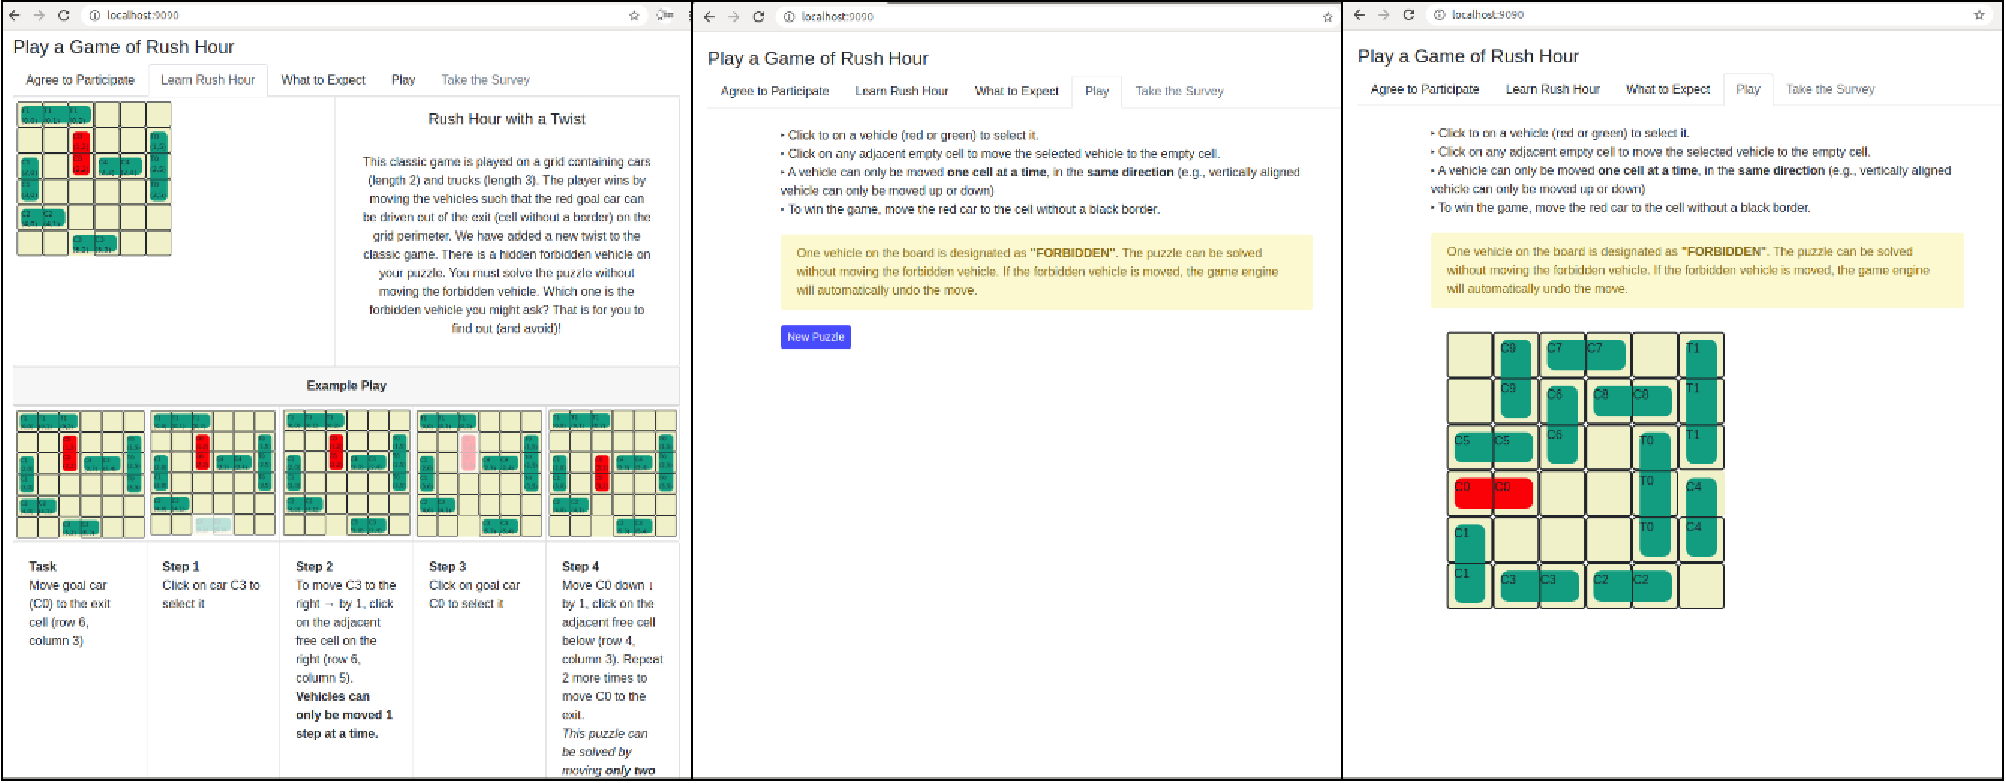
\includegraphics[width=\columnwidth]{img/UI.pdf}
  \caption{Rush Hour Simulation Framework Web Interface}
  \label{fig:ui}
\end{figure}



\subsection*{Collecting Data}
\textbf{Phase 1 - Without Intervention}\\
For each participant, we collect the solution to the Rush Hour puzzle and the demographic information. Data collection is complete. Data analysis is now in progress.

\textbf{Phase 2 - With Intervention}\\
For each participant, we will collect the user's solution to the Rush Hour puzzle, the demographic information and the rating for helpful tips in a 5-point Likert scale. This phase is not complete.

\subsection*{Experimental Design}
\textbf{Phase 1 - Without Intervention}\\
In the first phase of the study, the application user solves the puzzle without any intervention. Upon agreeing to participate in the study each subject is randomly assigned one puzzle out of ten puzzles. When the puzzle is solved, the subject is directed to complete the post-survey. We did not place any time restriction for the puzzle solving task. Participants were informed that one of the vehicles on the game board is forbidden and the puzzle must be solved without moving the forbidden vehicle. However, in this phase we did not give any visual cues (error messages, blocks) to the user in case they happen to move the forbidden vehicle during game play. 

We conducted a pilot study using nine graduate students to assess whether the human solvers were able to solve the selected puzzles within a reasonable amount of time. The pilot study participants solved their assigned puzzles within 5 - 10 minutes. The pilot study participants were also interviewed informally to get their perception of the puzzle difficulty. The participants commented that the puzzles were ''\textit{challenging}'' and "\textit{forced me to think}".

\textbf{Phase 2 - With Intervention}\\
In the second phase, the application intervenes the user and provides helpful hints. Upon agreeing to participate in the study each subject is assigned one puzzle randomly out of 13 puzzles (10 from phase 1 plus 3 new puzzles). In addition the participants are randomly selected to watch a 44 second video of a sample game play. During the game play, the participant is shown five hint types. The participant can follow a hint or decide to ignore it. Once the puzzle solving task is completed, the participants are asked to complete a short survey to capture the demographics and also asks them to subjectively rate the helpfulness of each hint type on a 5-point Likert scale. 

\subsubsection*{Participants}
\textbf{Phase 1 - Without Intervention}\\
We recruited subjects from a graduate and undergraduate university student population. 136 participants completed the study. The sample comprised of college undergraduate and graduate students in Computer Science, Psychology, Agriculture and Business majors. 117 of the 136 participants also completed the demographics survey.

\textbf{Phase 2 - With Intervention}\\
We will recruit subjects from a graduate and undergraduate university student population.

\subsubsection*{Summary of Findings}
\textbf{Phase 1 - Without Intervention}\\
Majority of the participants (39) were below the age of 20, while 38 subjects were between the age 20-25. Maximum age was 41 years. 70 of the 117 participants were male. When asked if they liked puzzle solving tasks, 78\% of the participants either agreed or strongly agreed with the statement. Specifically to the Rush Hour game 79\% of the participants liked or strongly liked Rush Hour. The most common reason as to why the participants liked puzzle solving tasks was that puzzle solving stimulates critical thinking skills. 30\% of the participants usually did a puzzle solving task once a month, while 21\% of the participants solved a puzzle once a week.

When asked about strategies the participants used to solve difficult puzzles, 79\% of the group said that they kept trying until the puzzle was eventually solved, while 12\% of the participants said that they would ask for help.  Given a new puzzle that they have not seen before, if they get stuck while solving the puzzle, 26\% said that they would not like any outside help. 47\% of the participants said that they would like a suggestion/tip that would get them past the current situation. 15\% said that they would like a warning, which indicated that their current approach would lead to a dead-end. 8\% of the participants said that they would like a warning and an explanation to help them prevent getting stuck in the future.  

\begin{figure}[htb]
  \centering
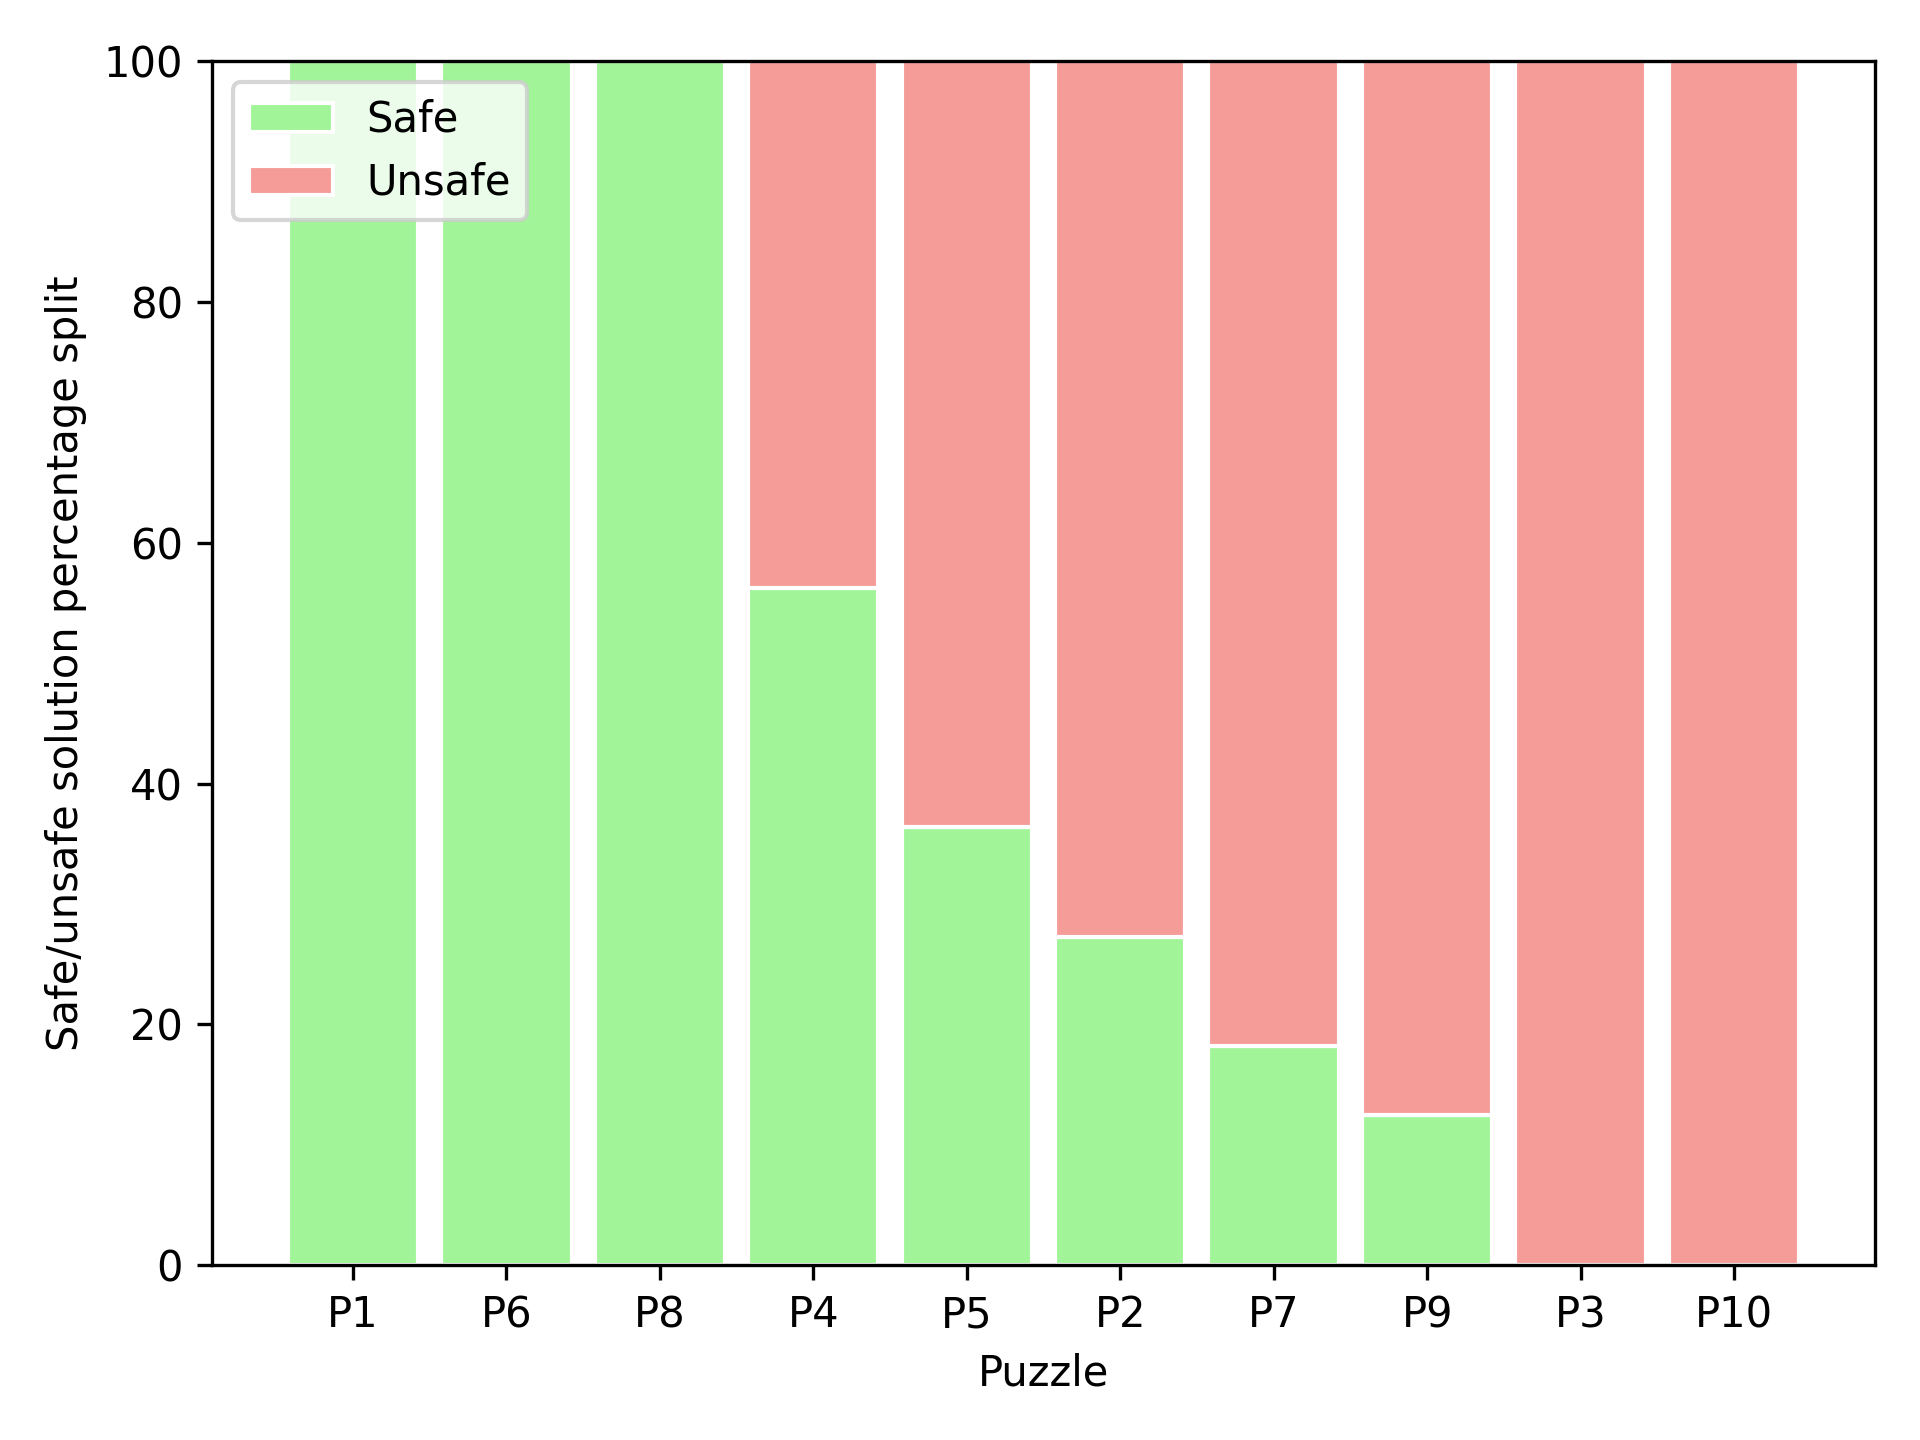
\includegraphics[width=0.5\columnwidth]{img/p2.png}
  \caption{Percentage split between unsafe and safe solutions produced by human users for puzzles P1 through P10}
  \label{fig:split}
\end{figure}


From the 136 subjects, 66 produced solutions that involved moving the forbidden vehicle. From those who moved the forbidden vehicle, 54 users moved the vehicle more than once. Mean number of moves was 53 ($SD=55$) for the sample and maximum number of moves was 378. Table \ref{tab:usersolutions} describes the summary statistics for safe and unsafe solutions produced by the human solvers. 

\begin{table}[htb]
\begin{tabular}{|l|l|l|l|l|l|l|l|l|l|l|}
\hline
\multicolumn{1}{|c|}{\multirow{2}{*}{PID}} &
  \multicolumn{5}{c|}{Safe Solutions} &
  \multicolumn{5}{c|}{Unsafe Solutions} \\ \cline{2-11} 
\multicolumn{1}{|c|}{} &
  \multicolumn{1}{c|}{Freq} &
  \multicolumn{1}{c|}{Min} &
  \multicolumn{1}{c|}{Max} &
  \multicolumn{1}{c|}{Mean} &
  \multicolumn{1}{c|}{SD} &
  \multicolumn{1}{c|}{Freq} &
  \multicolumn{1}{c|}{Min} &
  \multicolumn{1}{c|}{Max} &
  \multicolumn{1}{c|}{Mean} &
  \multicolumn{1}{c|}{SD} \\ \hline
P1  & 18 & 24 & 106 & 43.9  & 20.5  & -  & -  & -   & -    & -    \\ 
P2  &  3  & 44 & 158 & 99.3 & 57.1 & 8  & 78 & 378 & 190.3 & 120.0\\ 
P3  & -  & -  & -   & -     & -     & 12 & 25 & 50  & 35.5 & 8.3  \\ 
P4  & 9  & 23 & 46  & 30    & 7.1   & 7  & 25 & 124 & 67.4 & 33.9 \\ 
P5  & 4  & 23 & 32  & 26.5  & 3.9   & 7  & 14 & 82  & 32.0 & 23.3 \\
P6  & 14 & 22 & 55  & 29    & 10.3  & -  & -  & -   & -    & -    \\
P7  & 2  & 29 & 37  & 33    & 5.7   & 9  & 43 & 132 & 80.9 & 38.2 \\ 
P8  & 18 & 9  & 12  & 9.3   & 0.8   & -  & -  & -   & -    & -    \\
P9  & 2  & 21 & 27  & 24    & 4.2   & 14 & 29 & 169 & 66.3 & 39.0 \\
P10 & -  & -  & -   & -     & -     & 9  & 44 & 158 & 81.2 & 39.2 \\ \hline
\end{tabular}
\caption{Frequency, minimum, maximum, mean and std. deviation number of moves in users' solutions for the Rush Hour puzzles P1 through P10}
\label{tab:usersolutions}
\end{table}



\subsection*{Rush Hour Planning Domain Model}

We defined a domain model for the Rush Hour puzzle using PDDL (Planning Domain Definition Language). Constants of type direction in the domain model are used to identify movement directions right (\texttt{EW}), left (\texttt{WE}), down (\texttt{NS}), up (\texttt{SN}). The constants of type location identify cells in a $6 \times 6$ grid. The predicates are the state variables that may take the values \textit{True}/\textit{False}. The domain model consists of two actions \texttt{move-car} and \texttt{move-truck}. \texttt{move-car} action is described with the parameter set: car identifier ($C_i$), cell number of the starting position (\texttt{?from}), cell number of the end position (\texttt{?to}), the cell that becomes free after the move (\texttt{?tail}) and the direction of the move (\texttt{?d}). The action \texttt{move-truck} is defined similarly, the only difference being the truck's position is described by three cells (\texttt{?from}, \texttt{?mid}, \texttt{?to}). 

\begin{figure}[!ht]
\noindent\fbox{
 \parbox{\textwidth}{\raggedright: 
{\small
\texttt{(define (domain rush-hour)}\\
\texttt{\hspace*{35pt}(:requirements :strips :typing :universal-preconditions \\ 
\hspace*{35pt}:disjunctive-preconditions)}\\[15 pt]
        \hspace*{35pt}\texttt{(:types location vehicle direction)}\\ [15 pt]
        \hspace*{35pt}\texttt{(:constants  
                EW WE NS SN - direction \\
        \hspace*{35pt}L1 L2 L3 L4 L5 L6 L7 L8 L9 L10 L11 L12 L13 L14 L15 L16 L17 \\
        \hspace*{35pt}L18 L19 L20 L21 L22 L23 L24 L25 L26 L27 L28 L29 L30 L31 \\
        \hspace*{35pt}L32 L33 L34 L35 L36 - location)}\\[15 pt]
        \texttt{\hspace*{35pt}
        (:predicates \\
        \hspace*{35pt}(car ?v - vehicle)\\
        \hspace*{35pt}(truck ?v - vehicle)\\
    \hspace*{35pt}(at ?v - vehicle ?l - location)\\
        \hspace*{35pt}(face ?v - vehicle ?d - direction)\\
        \hspace*{35pt}(free ?l - location)\\
        \hspace*{35pt}(next ?d - direction ?l1 ?l2 - location)\\
        \hspace*{35pt})\\ [15 pt]}
\texttt{\hspace*{35pt}(:action move-car \\
                \hspace*{35pt}:parameters (?v - vehicle ?from ?to ?tail - location \\ \hspace*{35pt}?d - direction)\\
                \hspace*{35pt}:precondition (and (car ?v)(at ?v ?from)(at ?v ?tail)\\\hspace*{35pt}(face ?v ?d)(next ?d ?from ?to)(next ?d ?tail ?from)(free ?to))\\
                \hspace*{35pt}:effect (and (at ?v ?to) (not (at ?v ?tail))(free ?tail)\\\hspace*{35pt}(not (free ?to))))\\[15 pt]}
\texttt{\hspace*{35pt}(:action move-truck \\
                \hspace*{35pt}:parameters (?v - vehicle ?from ?to ?mid ?tail - location \\\hspace*{35pt}?d - direction)\\
                \hspace*{35pt}:precondition (and (truck ?v)(at ?v ?from)(at ?v ?mid)\\\hspace*{35pt}(at ?v ?tail)(face ?v ?d)(next ?d ?from ?to)(next ?d ?mid ?from)\\\hspace*{35pt}(next ?d ?tail ?mid)(free ?to))\\[0.25 pt]
                \hspace*{35pt}:effect (and (at ?v ?to)(at ?v ?from)(at ?v ?mid)\\\hspace*{35pt}(not (free ?from))(not (free ?mid))(not (at ?v ?tail))\\\hspace*{35pt}(free ?tail)(not (free ?to)))))
}
}
}
}
\caption{Rush Hour PDDL Domain Model}
\label{fig:domain}
\end{figure}

Table \ref{tab:plan} shows two plans for the Rush Hour puzzle illustrated in Figure \ref{fig:start}. The safe solution is obtained by an automated planner optimized for the number of moves. The unsafe (partial) solution is produced by a human user. The user's complete solution contains 43 moves. The highlighted step in the unsafe solution (18$^{th}$ move) is a dangerous move because it involves moving the forbidden vehicle \texttt{C2} for this puzzle. In the complete solution, the human user moved the forbidden vehicle twice.

\begin{table}[ht]
\begin{tabular}{|c|c|}
\hline
Safe solution (21 moves) & Unsafe solution (partial) \\
\hline
\begin{tabular}[c]{@{}l@{}}\texttt{\textsc{move-car c0 l17 l16 l18 we}}\\ \texttt{\textsc{move-car c0 l16 l15 l17 we}}\\ \texttt{\textsc{move-truck t3 l23 l17 l29 l35 ns}}\\ \texttt{\textsc{move-car c7 l20 l21 l19 ew}}\\ \texttt{\textsc{move-car c6 l25 l19 l31 ns}}\\ \texttt{\textsc{move-truck t1 l32 l31 l33 l34 we}}\\ \texttt{\textsc{move-car c5 l28 l34 l22 sn}}\\ \texttt{\textsc{move-truck t3 l17 l11 l23 l29 ns}}\\ \texttt{\textsc{move-car c7 l21 l22 l20 ew}}\\ \texttt{\textsc{move-truck t2 l14 l20 l8 l2 sn}}\\ \texttt{\textsc{move-truck t2 l20 l26 l14 l8 sn}}\\ \texttt{\textsc{move-truck t0 l3 l2 l4 l5 we}}\\ \texttt{\textsc{move-truck t3 l11 l5 l17 l23 ns}}\\ \texttt{\textsc{move-car c7 l22 l23 l21 ew}} \\ \texttt{\textsc{move-car c7 l23 l24 l22 ew}}\\ \texttt{\textsc{move-car c5 l28 l22 l34 ns}}\\ \texttt{\textsc{move-truck t1 l33 l34 l32 l31 ew}}\\ \texttt{\textsc{move-truck t1 l34 l35 l33 l32 ew}}\\ \texttt{\textsc{move-truck t2 l26 l32 l20 l14 sn}}\\ \texttt{\textsc{move-car c0 l15 l14 l16 we}}\\ \texttt{\textsc{move-car c0 l14 l13 l15 we}}\end{tabular} &
  \begin{tabular}[c]{@{}l@{}}\texttt{\textsc{move-car c0 l17 l16 l18 we}}\\ \texttt{\textsc{move-car c0 l16 l15 l17 we}}\\ \texttt{\textsc{move-car c4 l30 l24 l36 ns}}\\ \texttt{\textsc{move-car c4 l24 l18 l30 ns}}\\ \texttt{\textsc{move-truck t3 l23 l17 l29 l35 ns}}\\ \texttt{\textsc{move-truck t3 l17 l11 l23 l29 ns}}\\ \texttt{\textsc{move-truck t1 l34 l35 l33 l32 ew}}\\ \texttt{\textsc{move-truck t1 l35 l36 l34 l33 ew}}\\ \texttt{\textsc{move-car c7 l20 l21 l19 ew}}\\ \texttt{\textsc{move-car c6 l25 l19 l31 ns}}\\ \texttt{\textsc{move-truck t1 l34 l33 l35 l36 we}}\\ \texttt{\textsc{move-truck t1 l33 l32 l34 l35 we}}\\ \texttt{\textsc{move-truck t1 l32 l31 l33 l34 we}}\\ \texttt{\textsc{move-car c5 l28 l34 l22 sn}}\\ \texttt{\textsc{move-car c7 l21 l22 l20 ew}}\\ \texttt{\textsc{move-truck t2 l14 l20 l8 l2 sn}}\\ \texttt{\textsc{move-truck t2 l20 l26 l14 l8 sn}}\\ \colorbox{LightSalmon}{\texttt{\textsc{move-car c2 l9 l8 l10 we}}}\\ \texttt{\textsc{move-truck t0 l3 l2 l4 l5 we}}\\ \texttt{\textsc{move-truck t3 l11 l5 l17 l23 ns}}\\ \texttt{\textsc{move-truck t3 l17 l23 l11 l5 sn}}\\ \texttt{\textsc{move-truck t3 l23 l29 l17 l11 sn}}\\ $\ldots$\end{tabular} \\ \hline
\end{tabular}
\caption{A Solution Snippets for a Rush Hour Puzzle in Figure \ref{fig:start}}
\label{tab:plan}
\end{table}



If the puzzle configurations are viewed as nodes in a graph whose edges represent sequences of legal moves, finding a solution entails using a general graph search algorithm to find a path from the initial configuration to a goal configuration. However, the use of the STRIPS planning model allows us to exploit the powerful capabilities of an automated planner such as finding different plans using different optimization strategies (e.g., optimized by the number of moves, number of cars moved),  and finding alternative plans using different heuristics. Table \ref{tab:plan} shows two plans for the Rush Hour puzzle illustrated in Figure \ref{fig:start}. The safe solution is obtained by an automated planner optimized for the number of moves for the planning task $\Pi_{agent}$. The unsafe (partial) solution is produced by a human user. The user's complete solution contains 43 moves. The highlighted step in the unsafe solution (18$^{th}$ move) is a dangerous move because it involves moving the forbidden vehicle \texttt{C2} for this puzzle. In the complete solution, the human user moved the forbidden vehicle twice.

\begin{table}[ht]
\begin{tabular}{|c|c|}
\hline
Safe solution (21 moves) & Unsafe solution (partial) \\
\hline
\begin{tabular}[c]{@{}l@{}}\texttt{\textsc{move-car c0 l17 l16 l18 we}}\\ \texttt{\textsc{move-car c0 l16 l15 l17 we}}\\ \texttt{\textsc{move-truck t3 l23 l17 l29 l35 ns}}\\ \texttt{\textsc{move-car c7 l20 l21 l19 ew}}\\ \texttt{\textsc{move-car c6 l25 l19 l31 ns}}\\ \texttt{\textsc{move-truck t1 l32 l31 l33 l34 we}}\\ \texttt{\textsc{move-car c5 l28 l34 l22 sn}}\\ \texttt{\textsc{move-truck t3 l17 l11 l23 l29 ns}}\\ \texttt{\textsc{move-car c7 l21 l22 l20 ew}}\\ \texttt{\textsc{move-truck t2 l14 l20 l8 l2 sn}}\\ \texttt{\textsc{move-truck t2 l20 l26 l14 l8 sn}}\\ \texttt{\textsc{move-truck t0 l3 l2 l4 l5 we}}\\ \texttt{\textsc{move-truck t3 l11 l5 l17 l23 ns}}\\ \texttt{\textsc{move-car c7 l22 l23 l21 ew}} \\ \texttt{\textsc{move-car c7 l23 l24 l22 ew}}\\ \texttt{\textsc{move-car c5 l28 l22 l34 ns}}\\ \texttt{\textsc{move-truck t1 l33 l34 l32 l31 ew}}\\ \texttt{\textsc{move-truck t1 l34 l35 l33 l32 ew}}\\ \texttt{\textsc{move-truck t2 l26 l32 l20 l14 sn}}\\ \texttt{\textsc{move-car c0 l15 l14 l16 we}}\\ \texttt{\textsc{move-car c0 l14 l13 l15 we}}\end{tabular} &
  \begin{tabular}[c]{@{}l@{}}\texttt{\textsc{move-car c0 l17 l16 l18 we}}\\ \texttt{\textsc{move-car c0 l16 l15 l17 we}}\\ \texttt{\textsc{move-car c4 l30 l24 l36 ns}}\\ \texttt{\textsc{move-car c4 l24 l18 l30 ns}}\\ \texttt{\textsc{move-truck t3 l23 l17 l29 l35 ns}}\\ \texttt{\textsc{move-truck t3 l17 l11 l23 l29 ns}}\\ \texttt{\textsc{move-truck t1 l34 l35 l33 l32 ew}}\\ \texttt{\textsc{move-truck t1 l35 l36 l34 l33 ew}}\\ \texttt{\textsc{move-car c7 l20 l21 l19 ew}}\\ \texttt{\textsc{move-car c6 l25 l19 l31 ns}}\\ \texttt{\textsc{move-truck t1 l34 l33 l35 l36 we}}\\ \texttt{\textsc{move-truck t1 l33 l32 l34 l35 we}}\\ \texttt{\textsc{move-truck t1 l32 l31 l33 l34 we}}\\ \texttt{\textsc{move-car c5 l28 l34 l22 sn}}\\ \texttt{\textsc{move-car c7 l21 l22 l20 ew}}\\ \texttt{\textsc{move-truck t2 l14 l20 l8 l2 sn}}\\ \texttt{\textsc{move-truck t2 l20 l26 l14 l8 sn}}\\ \colorbox{LightSalmon}{\texttt{\textsc{move-car c2 l9 l8 l10 we}}}\\ \texttt{\textsc{move-truck t0 l3 l2 l4 l5 we}}\\ \texttt{\textsc{move-truck t3 l11 l5 l17 l23 ns}}\\ \texttt{\textsc{move-truck t3 l17 l23 l11 l5 sn}}\\ \texttt{\textsc{move-truck t3 l23 l29 l17 l11 sn}}\\ $\ldots$\end{tabular} \\ \hline
\end{tabular}
\caption{A Solution Snippets for a Rush Hour Puzzle in Figure \ref{fig:start}}
\label{tab:plan}
\end{table}



\begin{figure}[!ht]
  \centering
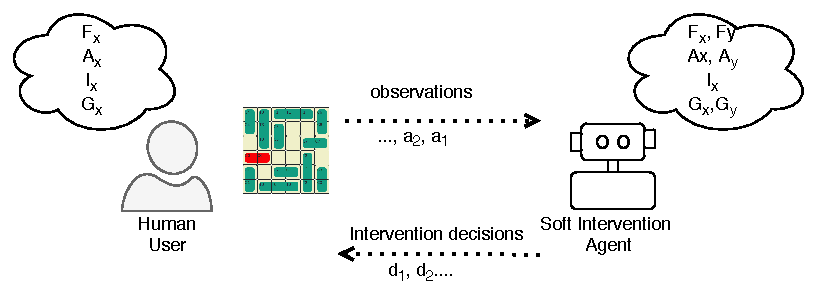
\includegraphics{img/model.pdf}
  \caption{The Soft Intervention Model}
  \label{fig:model}
\end{figure}
The planning problem for the soft intervention model develops around two actors: the human user and the intervention agent. As illustrated in Figure \ref{fig:model}, the human user's planning task is defined as: $\Pi_{user}=\langle F_x, A_x, I_x, G_x\rangle$, where $F_x$ is grounded with objects $\mathcal{O}\setminus o_f$, and $A_x \subseteq A_d$. $I_x$ is the initial board configuration and grounded with $\mathcal{O}$, which means the forbidden object is also available in the user's domain model. $G_x$ is the goal specification where predicates corresponding to car $C0$ being at the exit become \textit{True} in the state. User's solution to $\Pi_{user}$ generates an action sequence $\lbrace a_1, a_2, \ldots \rbrace$, which corresponds to the user's plan $\pi_{user}$. The intervention agent's domain model is different from the human user's because the agent knows about $o_f$. The intervention agent's planning task is defined as: $\Pi_{agent}=\langle \lbrace F_x\cup F_y\rbrace, \lbrace A_x \cup A_y\rbrace, I_x, (G_x\otimes G_y)\rangle$ where $F_x, A_x, I_x, G_x$ are defined as before. $F_y$ is grounded with $o_f$, and $A_y \subseteq A_u$. $G_y\subset F_y$ is the undesirable state. The agent's solution to $\Pi_{agent}$ is a plan $\pi_{agent}$. We use $\otimes$ symbol to denote that the agent needs to solve the planning problem for $G_x$, which \textit{avoids} $G_y$. In other words, any sub-plan (i.e, a sub sequence of actions) in $\pi_{agent}$ must not reach the state $G_y$.

User's actions have a cost that assigns a non-negative value to the action schema defined in the STRIPS domain definition. The cost function is given as $C: Op \rightarrow \mathbb{R}^0_+$. The cost of user's plan $c(\pi_{user})$ is  $\sum(c(a_i))$. The optimal solution, the optimal plan $\pi^*_{user}$, minimizes the cost. In this work, we assume all actions are uniform cost equal to 1.

When the user and the agent interact in real life, if the agent were to solve $\Pi_{agent}$, it would rely on an automated planner, which uses a variety of heuristics and optimizations. Because of this, a solution (or set of solutions) obtained by an automated planner may not match with the plan the user is producing. In intervention model we are proposing, the agent's role is to guide the user toward the goal and not directly solve the puzzle on the user's behalf. To do this, the agent needs to evaluate the user's plan up to now (a partial plan) to identify future problems. Our intervention design requires the agent to receive the user's actions as observations one at a time. Then the agent makes the decision to intervene having considered behavior properties of all observations made up to the current point. Our soft intervention model learns to recognize partial plans that may become unsafe in the future using these behavior properties. When the user makes a move on the puzzle, the intervention agent looks $k$ steps ahead into the future ($k \in \lbrace1,2,3\rbrace$) and decides whether or not the user will reach the undesirable state at step $k$. If the decision is yes, intervention takes place in the current step.
 
\subsubsection*{Assumptions About the Domain}
For the learned models developed from the results of this study, we make the following assumptions about the human user's planning problem for the Rush Hour domain.
\begin{description}
\item [User wants to avoid the undesirable state:]
In the scenarios we are modeling in this study, the need for intervention occurs when there is a mismatch between the human user's knowledge of the domain and the intervening agent's knowledge, and this discrepancy leads the user to an undesirable consequence. In the case of the Rush Hour domain, the user not being aware of the forbidden car creates an opportunity for the user to inadvertently commit to solutions that triggers the undesirable consequence. In the Rush Hour domain, we assume that the user does not behave as an adversary and attempt to willingly trigger the undesirable state. The adversarial case, in which  the environment contains an opponent (human/software agent) in addition to the human user and the intervention agent, is an interesting extension to the intervention problem and is applicable in many real-life domains such as cyber security and multi-player games.
\item [Knowledge of $G_x, G_y$:] 
We assume that the user is aware of the goal of the puzzle (i.e, move the red car to the exit) $G_x$ and actively pursues the goal. The user also welcomes the intervention decisions generated by the intervention agent. The user does not know the undesirable state $G_y$ but has the knowledge that it exists. The agent knows both $G_x$ and $G_y$.
\item [Actions are Deterministic and discrete:]
We assume that each action the user executes has only one outcome. The effect of the action is a discrete and instantaneous update of the state (vehicle positions) on the board.
\item [Observability:]
We assume that the user's actions (puzzle moves) are fully observable to the intervening agent.
\end{description}

\section*{The Rush Hour Web Simulator}
\subsection*{System Design Decisions}
We designed the Rush Hour software framework for conducting human subject studies in an environment that allows the user to be engaged in a cognitively taxing task. Our first design choice was in establishing the physical setup of the system. Because the experiments are targeted toward all kinds of computer software users (experts/non-experts), we wanted the subjects' attention to be mainly on the puzzle solving task and not be distracted by a complex user-interface. To allow for more users to participate, while minimizing the time commitment and the effort, we wanted the system to be accessible from anywhere (e.g, home, university etc.). Because of these reasons we designed the system to be a single page web application.
Our next design decision is concerned with capturing and storing experiment data. As per the university Institutional Review Board (IRB) regulations, the subject data is required to be stored in a secure manner. Further, because our system is deployed as a web application, multiple users may use the system at once and we need to ensure the data is transferred from the web application client to the server securely. We established communication between the client and the server over HTTPS via a stateless request-response scheme. The client side uses NodeJS, an asynchronous, event-driven JavaScript run-time, which is designed to build scalable network applications.  The client also uses NodeJS security modules (Helmet) for improved security. The data is stored in a secure remote, server dedicated to the web application. The design of the system needs to facilitate seamless transition between the two operating modes: learning behavior patterns that can be used as indicators of users' needing help and evaluating learned intervention models in situ. Therefore,  we designed the web application to interact with micro-services via a RESTful API. Our system architecture is RESTful, in the sense that the client interacts with the server by sending HTTP GET and POST requests using JSON messages to an endpoint URL in the server. The API defines many services (persisting game state, intervention, providing hints etc.). These services are implemented as separate components on the server. REST API response payloads sent from the server are text and encoded in JSON. The response is parsed at the client and appropriate event is triggered on the user interface. In addition to supporting platform-independence, which encourages user participation, the services can be activated and deactivated based on the operational mode. This allows us to extend the existing system to evaluate how human users respond different intervention models in the future.

\subsection*{System Architecture}
The basic system architecture is a JavaScript single page web application in an HTML5 browser that uses RESTful API to access micro-services provided by a Java server running on Linux. The client consists of a minimal index.html file that loads and executes the bundled JavaScript application. The client and server files are bundled into a single JAR file for the execution on the Linux server at a specified port. Figure \ref{fig:architecture} illustrates the system architecture.

\begin{figure}[!ht]
  \centering
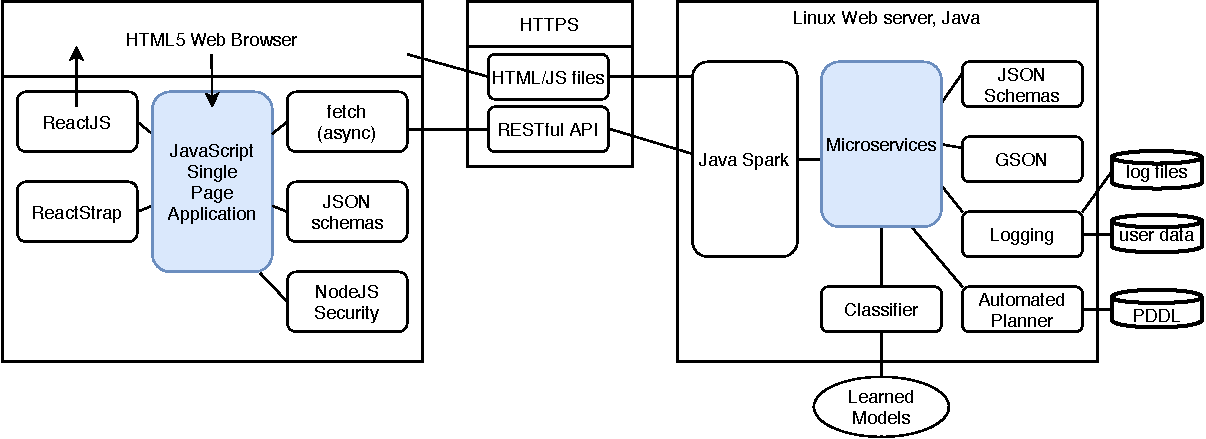
\includegraphics[width=\columnwidth]{img/architecture.pdf}
  \caption{The Client-Server Architecture of the Intervention System}
  \label{fig:architecture}
\end{figure}
The system is a client-server application that communicates over HTTPS. On the client side, the browser loads the index.html file, which in turn loads the bundled JavaScript single page application bundle.js. The single page application makes RESTful API requests to the server on the same port using JavaScript's asynchronous fetch. We defined several JSON schema to enable message passing between the client and the server via the RESTful API. The JSON schema verify requests on the server side and responses on the client side. Any verification failures are handled by error responses, also defined in the JSON schema. ReactJS renders the application using ReactStrap on the client. Because the communication between the client and the server occurs over the Internet, we use the NodeJS security module Helmet to secure the HTTP headers to prevent attacks like cross-site scripting.

On the server side, GSON is used to convert the JSON requests from the client to Java objects and Java objects to JSON responses. The server uses Java logging to record user data (moves, survey responses on the client side) and errors that occur on the server side on text files. The classifier and the automated planner components are activated only when evaluating learned intervention models. The automated planner component uses PDDL problem and domain definitions to retrieve information about the planning problem to help guide the user. The classifier component uses machine learning models to decide whether the user's partial solution requires intervention or not.

In the first mode of the operation, the application allows the user to solve the puzzle without any intervention. In this mode, the user interacts with four components: (1) consent agreement, (2) Rush Hour Tutorial, (3) Solver (Board), and (4) Post-study survey/Debriefing. The components are displayed as tabs on the web page. As the subject interacts with each of these components, unique API calls are triggered to inform the server about the status of the game. The consent agreement component lets the subject read the terms and conditions of the study and give informed consent to participate in the study as required by the IRB. When the user gives consent to participate in the study, the user gets assigned a unique identifier and components 2 and 3 get activated. This unique identifier is maintained at both the client side (as the Local Storage entry in the Web browser) and on a text file at the server until the user's session ends. The Rush Hour tutorial presents a brief introduction to the Rush Hour puzzle, the rules and the objective of the puzzle. It also shows an example play to educate the user on how to select and move objects on the web interface. Components 1 and 2 are static components, in the sense the user does not have a lot of flexibility to change the contents through interaction. On the other hand, the solver is a dynamic and an interactive component. The solver component allows the user to start a puzzle solving task by clicking a button, at which point a random Rush Hour puzzle is fetched from the server. The participant can move the vehicles on the grid by first clicking once on the vehicle to select it and then clicking once on an adjacent empty cell to move it to the selected cell. To comply with the classical planning model of discrete actions, the application forces the user to move the vehicles one step at a time. This rule invalidates moves that jump over multiple cells on the puzzle boards. The other illegal move is user attempting to move a vehicle in the opposite orientation. When the user makes one of these illegal moves, error messages are displayed and the move is blocked. All legal moves the user make are temporarily kept in in-memory data structures on the client side. Once the user finishes the puzzle solving task, an API call is invoked to initiate the data transmission between the client and the server in a secure manner via HTTPS. The server records the users solution on a text file in a directory created with the user's identifier. When the user's solution is stored on the server successfully, component 4 gets activated. The post-study survey in this mode, collects demographic data and the user's general puzzle solving habits. Once the user completes the survey, the data is transmitted to the server to be stored similar to the data storage protocol used in component 3.

\begin{figure}[!hbt]
  \centering
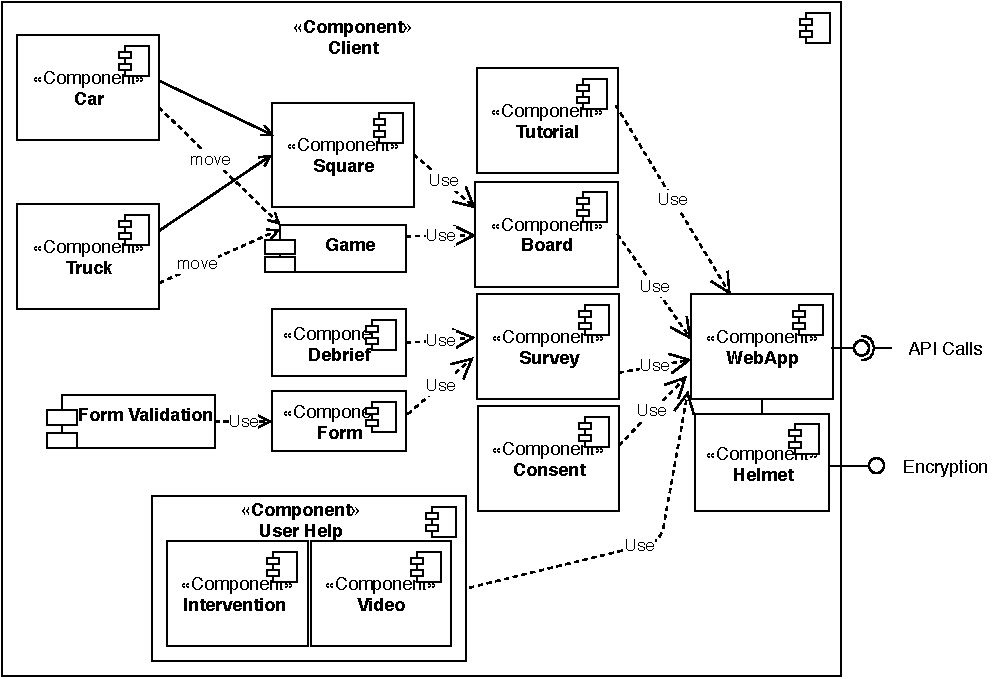
\includegraphics[width=\columnwidth]{img/componentclient.pdf}
  \caption{UML Component Diagram for the Intervention System Client}
  \label{fig:compclient}
\end{figure}

Figure \ref{fig:compclient} illustrates the component structure of the intervention client used in the second mode of operation, which uses intervention. In this mode, the user interacts with five components on the client side: (1) consent agreement, (2) Rush Hour Tutorial, (3) Solver, (4) User Help and (4) Post-study survey/Debriefing. Components 1, 2, 3, and 5 function similar to the first operation mode. The User Help component is used to communicate intervention decisions from the server and the subsequent user responses. In this study we evaluate the effects of offering help before the user starts the puzzle solving task and during. Video component supports the former, which plays a 45 second video clip on how to solve an example puzzle. The video is played to randomly selected users to simulate an experiment condition. The intervention component supports intervention decisions during the play. The communication model between the client and the server differ from the first operation mode, in that in addition to retaining users' moves in memory, each puzzle move the user makes invokes an API call to the server to retrieve an intervention decision. If intervention occurs, the Intervention component displays a pop-up dialog box with five help options. When the user requests one of the help options, the client makes another API call to fetch a response from the server. The response is displayed as a follow up dialog box and the user is allowed to continue on with the puzzle solving task. Figure \ref{fig:help} shows the intervention message shown to the user (left) and  the user requesting to see the next best move and the subsequent response from the server displayed for the user (right). One of the help options is to let the user ignore intervention. The intervention component keeps track of how many times the user has chosen to ignore intervention and after two consecutive ignore requests, the client terminates fetching intervention responses from the server. When the puzzle solving task finishes, the user's solution and different responses to intervention decisions are transmitted to the server for persistence.

\begin{figure}[!hbt]
  \centering
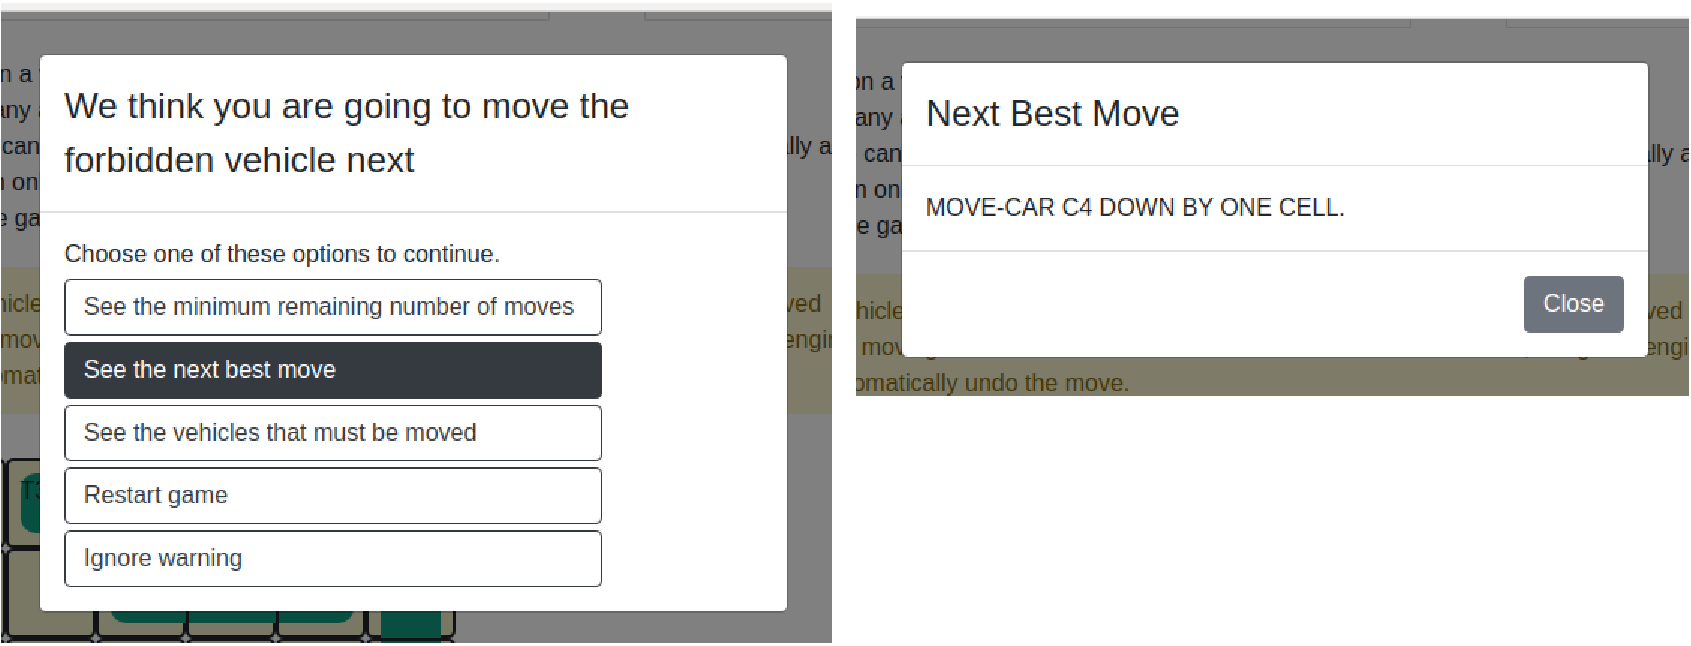
\includegraphics[width=\columnwidth]{img/alert.pdf}
  \caption{Intervention Step and Help}
  \label{fig:help}
\end{figure}
As shown in Figure \ref{fig:compserver}, the server responds to client's API calls through the micro-server. The intervention component and the planning component in the server are used to identify when the user needs help and generate helpful hints respectively. The intervention component uses a classifier to identify behavior features in the user's solution. The planning component responds to user's responses to intervention decisions by generating optimal plans and landmarks for the Rush Hour planning problem.

\begin{figure}[!hbt]
  \centering
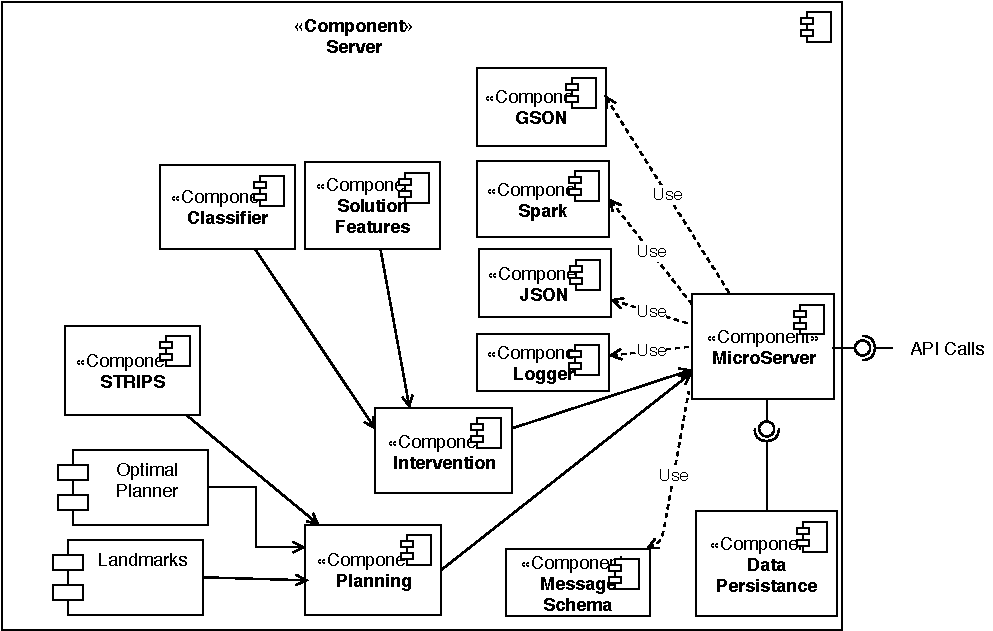
\includegraphics[width=\columnwidth]{img/componentserver.pdf}
  \caption{UML Component Diagram for the Intervention System Server}
  \label{fig:compserver}
\end{figure}

We use a minimalist and responsive design (supported by ReactStrap library) for the web application interface to help the user to start the puzzle solving task with a very small learning curve. The simple interaction model we designed for the users' to solve the puzzle and simultaneously communicate event data to the server helps the user focus completely on the puzzle solving task. The system is launched on a secure Linux web server with a public IP address, which allows the users to access the application from anywhere on a variety of devices. Figure \ref{fig:ui} shows the web application interface: the tutorial tab, play tab before the user starts the puzzle and when the puzzle is loaded in that order.
\begin{figure}[!hbt]
  \centering
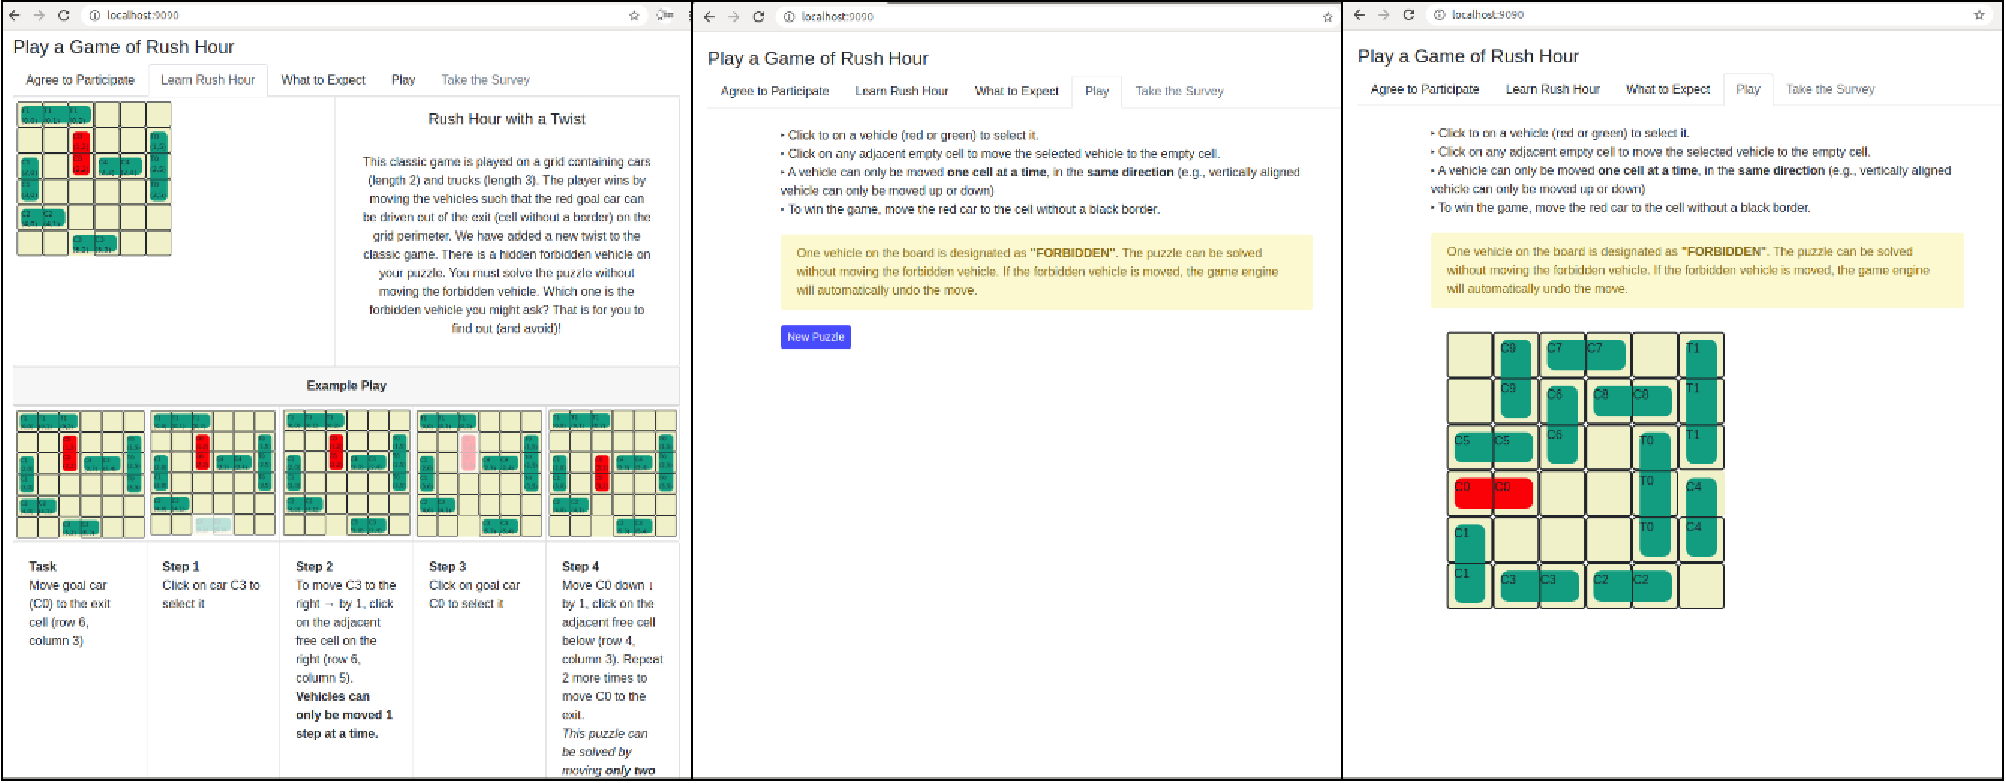
\includegraphics[width=\columnwidth]{img/UI.pdf}
  \caption{Rush Hour Simulation Framework Web Interface}
  \label{fig:ui}
\end{figure}
\subsection*{Rush Hour Puzzle Design Decisions}

When choosing Rush Hour puzzle configurations for the study, we want to carefully balance the puzzle's difficulty for a human user. Especially, given the PSPACE-completeness of the (generalized) puzzle, we need the puzzles to be solvable by human users in a reasonable time. Further, we use the Rush Hour puzzle as a supplementary task comparable to human users learning to use a new software or a web application. Therefore, the puzzle solving task should pose a sufficient challenge for the user during the search for a solution in order to make the intervention step more meaningful. We introduce a forbidden vehicle, which must not be moved to each puzzle to restrict the moves the user is allowed to make. This is an alternative way to increase the difficulty of the puzzle without having to increase the number of vehicles on the board \cite{fernau2003}. In order to further instill the importance of avoiding the forbidden vehicle in the user's mind, we also provided warning messages on the Web interface (see the yellow information bar in Figure \ref{fig:ui} panel 2/3) to inform the user about the presence of a forbidden vehicle and what will happen should the forbidden car was moved. However, the users are not explicitly informed what the specific forbidden vehicle is, unless the user moves it during game play. At that point, the user is first shown an alert message indicating that the forbidden vehicle was moved and the move will be undone.

In this study we use ten Rush Hour puzzles to produce learned models for soft intervention and three additional puzzles to evaluate the helpful hints. We classify these thirteen puzzles into three groups by the position of the forbidden vehicle. Figure \ref{fig:puzzles} shows the three puzzle types: type A has the forbidden vehicle in the corner of a grid, type B has the forbidden vehicle on the edge of the grid and type C has the forbidden vehicle in the middle of the grid. We hypothesize that these three types will pose unique challenges for the user to avoid the forbidden vehicle. To produce the learned models, we use four puzzles of type A, five puzzles of type B and one puzzle of type C. To evaluate helpful hints, we use four puzzles from types A, C and five puzzles from type B. Table \ref{tab:puzzles} shows the puzzle assignments used to produce learned models (10 puzzles) and evaluate hints (13 puzzles). $Pi, i=\lbrace 1,\ldots,13 \rbrace$ indicate the puzzle identifier.

\begin{figure}[!hbt]
  \centering
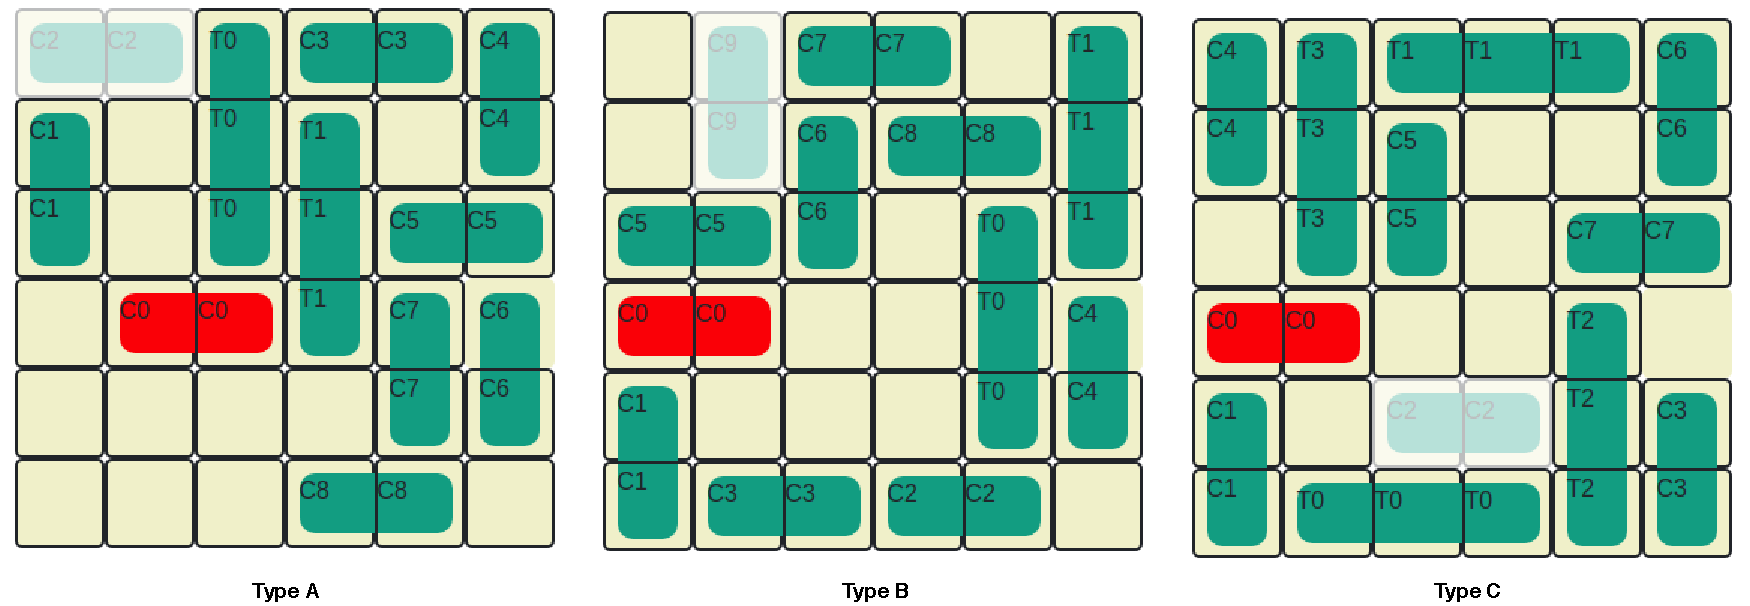
\includegraphics[width=\columnwidth]{img/puzzles.pdf}
  \caption{Rush Hour puzzle configuration types with forbidden vehicles highlighted}
  \label{fig:puzzles}
\end{figure}

\begin{center}
\begin{table}
\begin{tabular}{ll}
\begin{tabular}{|c|c|}
\hline
Type & Puzzles\\
\hline
A & P2, P4, P6, P8 \\
\hline
B & P1, P3, P5, P9, P10 \\
\hline
C & P7 \\
\hline
\end{tabular}
\quad
\begin{tabular}{|c|c|}
\hline
Type & Puzzles\\
\hline
A & P2, P4, P6, P8 \\
\hline
B & P1, P3, P5, P9, P10 \\
\hline
C & P7, P11, P12, P13 \\
\hline
\end{tabular}
\end{tabular}
\caption{Rush Hour puzzle assignment for learning intervention (left) and evaluating hints (right)}\label{tab:puzzles}
\end{table}
\end{center}

\section*{Learning Soft Intervention} %Phase 1
When the user solves a puzzle, the intervening agent receives the vehicle moves as a series of observations $\mathcal{M}=\lbrace m_1, m_2, \ldots \rbrace$, and $\mathcal{M} \subseteq \mathcal{A}$. Given $\mathcal{M}$, an initial state $I$, puzzle goal state $G_x$, and an undesirable state to avoid $G_y$, the soft intervention problem is defined as a tuple $\Xi=\lbrace \mathcal{M}, I, G_x, G_y\rbrace$. Execution of $\mathcal{M}$ is defined using the state transition function $\delta$ recursively as follows:

\begin{definition}
The execution of a sequence of linearly ordered actions $\mathcal{M}$ of length $l$ ($|\mathcal{M}|=l$) from the initial state $I$ results in a state $s$ defined by the function: $\Delta (I, \mathcal{M}) = \delta( \ldots \delta(\:\delta(I,m_1),\:m_2) \ldots, m_l)$
\end{definition}

Note that $\mathcal{M}$ is only a partial solution for the puzzle solving task $\Pi_{user}$ and $\Delta (I, \mathcal{M}) \not\models G_x$. The intervening agent needs to decide to intervene or not for a partial solution $\mathcal{M}^F, |\mathcal{M}^F|=k$ and $k>l$. In other words, the agent predicts whether or not the user will reach $G_y$, ($k-l$) steps into the future. For this work we restrict the interval of $(k-l)=[1,3]$. Therefore, we represent the \textit{soft intervention problem} for the Rush Hour puzzle as a binary classification problem. Formally, the solution to the soft intervention problem is a function $\mathcal{I}$ such that, given a $N$-dimensional input vector $x \in \mathcal{X} \subseteq \mathbb{R}^N$, $x$ is mapped to a set of fixed classes $C$:

\begin{equation}
\mathcal{I} : \mathcal{X} \to C=\lbrace Yes, No\rbrace
\end{equation}

The label \textit{Yes} indicates that the human user needs help and must be intervened, while the \textit{No} label indicates that the human user should not be intervened. In the supervised mode, $\mathcal{I}$ is learned by observing actual examples of human users solving Rush Hour puzzles. We denote the supervised learning method by $T$ and $T(D)=\mathcal{I}$. The learning method $T$ takes a training set $D$ as input and returns the learned classifier function $\mathcal{I}$. We explore five learning methods in this study: $\mathcal{I} \in \lbrace $ Decision Tree, Random Forest, k-nearest neighbor, Logistic Regression, Naive Bayes $\rbrace$  $D$ is a set of labeled game plays $\langle g, c\rangle$ where $\langle g, c\rangle$ $\in X \times C$. 

We want to transform the user's game play $g$ into a representation of $x$ that allows us to capture where the user is in the state space of the Rush Hour planning problem at the time the decision to intervene is made and  produce measurable attributes that describe how the user has been exploring the state space. For example, is the user advancing toward the winning state by making helpful moves?, is the user currently exploring a risky part in the state space and getting closer to the undesirable state? We hypothesize that behavior patterns as these have a correlation to the event of the user moving the forbidden vehicle and these patterns can be used to as features of a learning method to recognize in advance if the user needs intervention. We designed a human subject experiment to identify common behavior patterns.

\subsection*{The Human Subject Experiment}
\subsubsection*{Experimental Design}
As shown in Table \ref{tab:puzzles}, we created ten unique Rush Hour puzzles. We conducted a pilot study using nine graduate students to assess whether the human solvers were able to solve the selected puzzles within a reasonable amount of time. The pilot study participants solved their assigned puzzles within 5 - 10 minutes. The pilot study participants were also interviewed informally to get their perception of the puzzle difficulty. The participants commented that the puzzles were ''\textit{challenging}'' and "\textit{forced me to think}". The same puzzles used in the pilot were used in the actual study.

For the actual study, we recruited subjects from a graduate and undergraduate university student population. The participants were not compensated for their time. After obtaining informed consent, the participants were directed to the Web URL, which hosted the Rush Hour simulator software. Each participant was assigned to solve one Rush Hour puzzle randomly selected from a set of ten. We did not place any time restriction for the puzzle solving task. Participants also had the option to use an online tutorial (available on the simulator itself) on how to play the Rush Hour puzzle. All ten puzzles contained a forbidden vehicle. Participants were informed that one of the vehicles on the game board is forbidden and the puzzle must be solved without moving the forbidden vehicle. However, in this phase we did not give any visual cues (error messages, blocks) to the user in case they happen to move the forbidden vehicle during game play. Once the puzzle solving task was completed, the participants were asked to complete a short demographic survey on their general puzzle solving habits. Figure \ref{fig:phase1} illustrates the activity sequence of the experiment. 136 participants completed the study. The sample comprised of college undergraduate and graduate students in Computer Science, Psychology, Agriculture and Business majors. 117 of the 136 participants also completed the demographics survey.

\begin{figure}[!hbt]
  \centering                                                    
  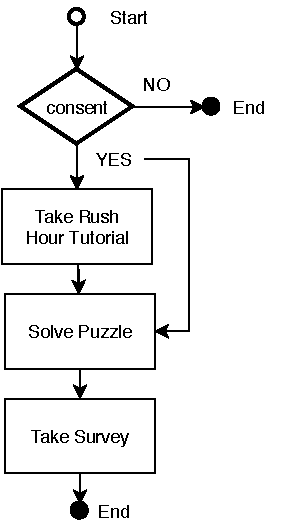
\includegraphics[keepaspectratio]{img/phase1.pdf}
  \caption{Activity sequence for learning when to intervene human subject experiment}
  \label{fig:phase1}
\end{figure}

\subsubsection*{Findings - Demography Survey}
Majority of the participants (39) were below the age of 20, while 38 subjects were between the age 20-25. Maximum age was 41 years. 70 of the 117 participants were male. When asked if they liked puzzle solving tasks, 78\% of the participants either agreed or strongly agreed with the statement. Specifically to the Rush Hour game 79\% of the participants liked or strongly liked Rush Hour. The most common reason as to why the participants liked puzzle solving tasks was that puzzle solving stimulates critical thinking skills. 30\% of the participants usually did a puzzle solving task once a month, while 21\% of the participants solved a puzzle once a week.

When asked about strategies the participants used to solve difficult puzzles, 79\% of the group said that they kept trying until the puzzle was eventually solved, while 12\% of the participants said that they would ask for help. 

Given a new puzzle that they have not seen before, if they get stuck while solving the puzzle, 26\% said that they would not like any outside help. 47\% of the participants said that they would like a suggestion/tip that would get them past the current situation. 15\% said that they would like a warning, which indicated that their current approach would lead to a dead-end. 8\% of the participants said that they would like a warning and an explanation to help them prevent getting stuck in the future.  The most common medium for solving puzzles was using their mobile devices (42\%). 31\% of the participants used the personal computers/laptops to solve puzzles. 19\% of the participants solved puzzles using physical means (e.g., puzzle books, newspapers and physical puzzles such as Rubik's  cubes)

\subsubsection*{Findings - Avoiding Forbidden Vehicle}
The Rush Hour search problem can be optimized using two parameters: (1) number of moves and, (2) number of vehicles moved. Defining the Rush Hour problem as a STRIPS planning problem allows us to use off-the-shelf planners (configured to use an admissible heuristic during search) to find solutions optimized to minimize both these parameters. Regardless the optimizing parameter, inclusion of the forbidden vehicle further classifies the optimal solutions into two categories: (1) safe - optimal solutions that do not contain forbidden vehicle moves and (2) unsafe - optimal solutions that contain forbidden vehicles moves. Optimal solution costs for all these categories of solutions are summarized in Table \ref{tab:optimals}. It can be seen that solution costs for safe and unsafe solutions for the ten puzzles optimizing for the minimum number of vehicles is identical. However, optimizing for the minimum number of moves we see that for puzzles P3 and P5, the unsafe solution costs less than the safe solution. This means that it is possible for the user to find a shorter solution for these two puzzles by moving the forbidden car. We used the HSP planner \cite{bonet01planningas} to find the optimal solutions.

\begin{table}[!htb]
\begin{tabular}{|l|c|c|c|c|}
\hline
\multirow{2}{*}{PID} & \multicolumn{2}{l|}{Number of Moves} & \multicolumn{2}{l|}{Number of Cars} \\ \cline{2-5} 
    & Safe & Unsafe & Safe & Unsafe \\ \hline
P1  & 24   & 24     & 8    & 8      \\ 
P2  & 30   & 30     & 10   & 10     \\ 
P3  & \textbf{35}   & \textbf{25}     & 10   & 10     \\ 
P4  & 23   & 23     & 9    & 9      \\ 
P5  & \textbf{21}   & \textbf{14}     & 7    & 7      \\ 
P6  & 22   & 22     & 8    & 8      \\ 
P7  & 21   & 21     & 8    & 8      \\ 
P8  & 9    & 9      & 5    & 5      \\ 
P9  & 21   & 21     & 10   & 10     \\
P10 & 24   & 24     & 9    & 9      \\ \hline
\end{tabular}
\caption{Optimal costs for the safe and unsafe Rush Hour solutions for puzzles P1 through P10, optimized for number of moves and number of cars}
\label{tab:optimals}
\end{table}

From the 136 subjects, 66 produced solutions that involved moving the forbidden vehicle. From those who moved the forbidden vehicle, 54 users moved the vehicle more than once. Mean number of moves was 53 ($SD=55$) for the sample and maximum number of moves was 378. Table \ref{tab:usersolutions} describes the summary statistics for safe and unsafe solutions produced by the human solvers. Figure \ref{fig:split} illustrates the percentage split between unsafe and safe solutions for each puzzle. All users who solved P1 (type A), P6 and P8 (both type B) avoided the undesirable state. Interestingly, examining the structure of P1, although it is type B, it can be seen that moving the forbidden vehicle makes the puzzle unsolvable. The users who solved P1 did not move the forbidden vehicle. 

\begin{figure}[htb]
  \centering
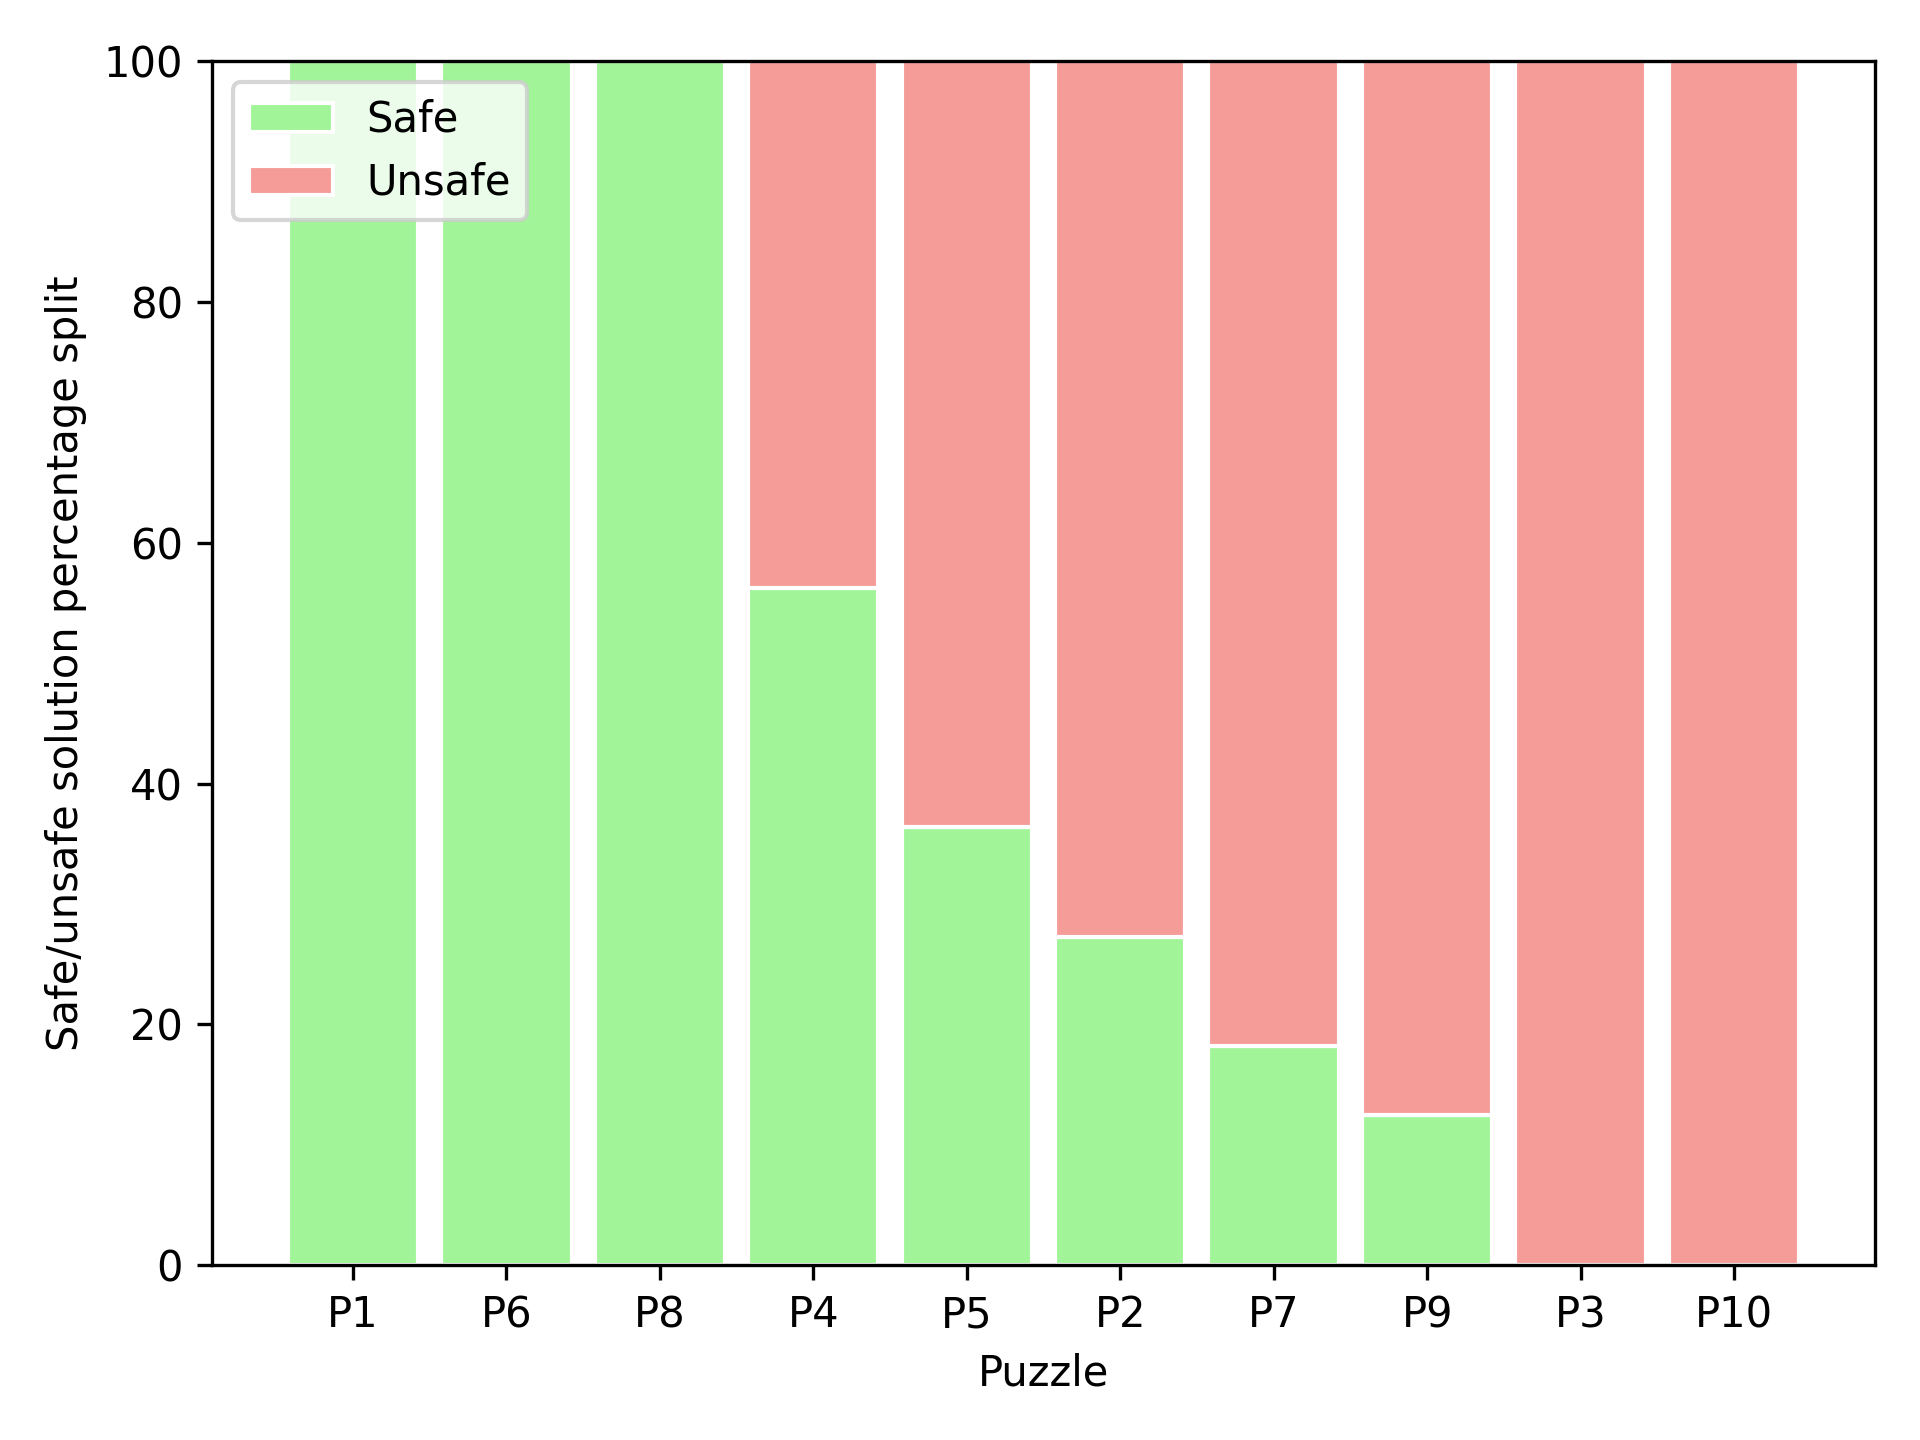
\includegraphics[width=0.5\columnwidth]{img/p2.png}
  \caption{Percentage split between unsafe and safe solutions produced by human users for puzzles P1 through P10}
  \label{fig:split}
\end{figure}
\begin{table}[htb]
\begin{tabular}{|l|l|l|l|l|l|l|l|l|l|l|}
\hline
\multicolumn{1}{|c|}{\multirow{2}{*}{PID}} &
  \multicolumn{5}{c|}{Safe Solutions} &
  \multicolumn{5}{c|}{Unsafe Solutions} \\ \cline{2-11} 
\multicolumn{1}{|c|}{} &
  \multicolumn{1}{c|}{Freq} &
  \multicolumn{1}{c|}{Min} &
  \multicolumn{1}{c|}{Max} &
  \multicolumn{1}{c|}{Mean} &
  \multicolumn{1}{c|}{SD} &
  \multicolumn{1}{c|}{Freq} &
  \multicolumn{1}{c|}{Min} &
  \multicolumn{1}{c|}{Max} &
  \multicolumn{1}{c|}{Mean} &
  \multicolumn{1}{c|}{SD} \\ \hline
P1  & 18 & 24 & 106 & 43.9  & 20.5  & -  & -  & -   & -    & -    \\ 
P2  &  3  & 44 & 158 & 99.3 & 57.1 & 8  & 78 & 378 & 190.3 & 120.0\\ 
P3  & -  & -  & -   & -     & -     & 12 & 25 & 50  & 35.5 & 8.3  \\ 
P4  & 9  & 23 & 46  & 30    & 7.1   & 7  & 25 & 124 & 67.4 & 33.9 \\ 
P5  & 4  & 23 & 32  & 26.5  & 3.9   & 7  & 14 & 82  & 32.0 & 23.3 \\
P6  & 14 & 22 & 55  & 29    & 10.3  & -  & -  & -   & -    & -    \\
P7  & 2  & 29 & 37  & 33    & 5.7   & 9  & 43 & 132 & 80.9 & 38.2 \\ 
P8  & 18 & 9  & 12  & 9.3   & 0.8   & -  & -  & -   & -    & -    \\
P9  & 2  & 21 & 27  & 24    & 4.2   & 14 & 29 & 169 & 66.3 & 39.0 \\
P10 & -  & -  & -   & -     & -     & 9  & 44 & 158 & 81.2 & 39.2 \\ \hline
\end{tabular}
\caption{Frequency, minimum, maximum, mean and std. deviation number of moves in users' solutions for the Rush Hour puzzles P1 through P10}
\label{tab:usersolutions}
\end{table}

\subsection*{Extracting Features}
We use the properties derived from the game state (positions of objects on the board) and the properties of the users' partial solution that has been observed up to now to extract features that correspond to the user's game play behavior. 
\subsubsection*{Game State}
We describe the game state using the \textit{vehicle positions} and  also their \textit{mobility}. With soft intervention, we hope to help the user reach the goal state, while avoiding the undesirable state. To this end, to learn the soft intervention model, instead of describing the positions of all the vehicles on the board, the features that capture the game state mainly focus on the positions of only the target vehicle (red color) and the forbidden vehicle and also their corresponding adjacent vehicles. We use the game state features associated with to the target car to measure how close the user is to the goal state. The features associated to the forbidden car evaluate how close the user is getting to triggering the undesirable state. Furthermore, we use a combination of raw feature values corresponding to the game state, as well as the abstractions of these features such as the mean and the frequency. This reduces the size of our input feature vector and at the same time gives us an estimate on where the user is in the state space; closer to moving the forbidden vehicle or advancing toward the goal state.

In general, the human solvers found it easier to avoid moving the forbidden vehicle in type A puzzles. Three of the four type A puzzles, had all or majority of human solvers managing to avoid the forbidden vehicle. Altogether, 83\% of subjects who solved type A puzzles avoided moving the forbidden vehicle. On the other hand, when the forbidden vehicle is on the perimeter of the board, type B, human solvers often moved the forbidden vehicle. In this case, only 36\% of the users who solved type B puzzles, managed to avoid moving the forbidden vehicle. All human solvers who attempted two puzzles of type B (P3, P10) moved the forbidden vehicle in their solutions. Ability to avoid moving the forbidden car dropped further for type C puzzles. The majority of the users (82\%) who attempted P7 (type C) moved the forbidden vehicle while solving the puzzle. This is intuitive because the forbidden vehicle in type C is the most exposed thus making the user less likely to correctly guess the forbidden car in advance.

Mobility of the two critical objects in the puzzle: target car and the forbidden vehicle, provide clues about the users' game state. As seen in the three puzzle types, more blocked the forbidden vehicle is the less likely the users are to move it. The objects on the path of the target car must first be moved out to clear the path. In doing so, the human user could move vehicles in such a way that the forbidden vehicle becomes free. In the initial configuration of the puzzles used for this experiment, the forbidden vehicles were blocked from all sides. Only puzzles P7 and P9 had the forbidden vehicles free in the initial configuration. We manually examined the human user solutions produced in this experiment to identify common movement patterns. We found that if the user was moving vehicles adjacent to the forbidden vehicle in such a way that the forbidden vehicle was freed, most users ended up moving it. This means that by monitoring the state changes that occur around the forbidden car, we can estimate whether the user will end up moving the forbidden vehicle or not. Similarly we capture the vehicle movements that take place on the target car's path to the exit, for example, the moves that result in reducing the number of vehicles blocking the target car is considered to be helpful to move the game state closer to the goal state.

Note that during a game play a human user can move the forbidden car multiple times because the simulator does not give any feedback in this experiment. When extracting features for the soft intervention model, we consider the partial solutions from the start to the point when the forbidden car was moved for the first time. In addition to the target and the forbidden vehicles, we introduce two additional critical vehicle sets: \textit{target car blockers} and \textit{forbidden car blockers}. Blockers are vehicles that are  directly on the path of another vehicle. Figure \ref{fig:blockers} illustrates an example board state. The target car's path is blocked by two vehicles C1 and T1. Therefore, \textit{target car blockers} $= \lbrace C1, T1\rbrace$. We only consider the vehicles that are between the target car and the exit cell as blockers because, only those vehicles are preventing the target car from reaching the goal state. The forbidden vehicle's movement is blocked by two vehicles C1 and C2. Therefore, \textit{forbidden car blockers} $=\lbrace C1, C2\rbrace$. We now describe the behavior features we designed considering the game state.

\begin{figure}[htb]
  \centering
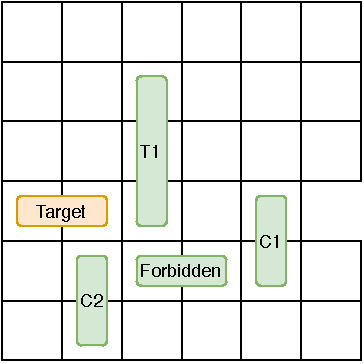
\includegraphics[width=0.35\columnwidth]{img/blockers.pdf}
  \caption{Blocker Vehicles}
  \label{fig:blockers}
\end{figure}
\begin{description}
\item[\texttt{blocks}:] number of times a move increased the number of cars blocking the target car's path
\item[\texttt{frees}:] number of times a move freed up empty spaces around the forbidden vehicle
\item[\texttt{freebci}:] number of times the number of empty spaces around the forbidden vehicle blockers increased
\item[\texttt{freebcd}:] number of times the number of empty spaces around the forbidden vehicle blockers decreased
\item[\texttt{freegci}:] number of times the number of empty spaces around the target car blockers increased
\item[\texttt{freegcd}:] number of times the number of empty spaces around around the target car blockers decreased
\item[\texttt{mgc}:] mean number of empty spaces around the target car blockers
\item[\texttt{mbc}:] mean number of empty spaces around the forbidden car blockers
\item[\texttt{reset}:] number of times the current move changed the state back to the initial puzzle configuration
\end{description}

\subsubsection*{Human Solvers' Partial Solutions}
The partial solutions the human users generate during game play provide clues to deciding whether or not the user will trigger the undesirable state. As seen in Table \ref{tab:usersolutions}, the mean number of moves for a safe solution (a solution that does not contain forbidden vehicle moves) is lower than the mean number of moves for an unsafe solution for the same puzzle. When we manually examined the human user solutions we found that the users who produced unsafe solutions often made unhelpful moves. For example, most of them moved the same vehicle back and forth many times in succession. For this study, we define one unhelpful move type called the \textit{h-step undo}.

\begin{definition}
Given a partial solution $\mathcal{M}=\lbrace m_1, m_2...m_i \rbrace$, $|\mathcal{M}|=i$, $\mathcal{M}\subseteq \mathcal{A}$ and initial state $I$, let state $s_i=\Delta(I,\mathcal{M})$. A h-step undo is a state transition such that $\Delta(s_i, \lbrace m_{i+1}, \ldots, m_h\rbrace)=s_i$ and $h>i$, $h \in \mathbb{N}$.
\end{definition}

The h-step undo is a move that takes the game state back to a previously seen state (i.e, an undo operation). In this work we only consider $h=1$, which asks the question did the current move just undo the move that happened immediately before?

Comparing the number of moves of the partial solution to that of an optimal solution is helpful in identifying whether the user is moving away from the goal state or making progress toward it. Here, we use the safe solution optimized for the number of moves. We used the HSP planner to find the optimal solution for each puzzle. Figure \ref{fig:difficuly} illustrates how the number of moves in users' solutions compare to a set of threshold values derived from the optimal solution. We define the threshold set $\theta$ as: given the optimal number of moves  $\alpha$ for a puzzle, $\theta=\lbrace \alpha, 1.2\times \alpha, 1.4\times \alpha, 1.6\times \alpha, 1.8\times \alpha\rbrace$. It can be seen that human solvers' solutions to P8 were very close to the optimal solution in the number of moves. Human solvers' found it very difficult to find a solution closer to the optimal number of moves for P2. Interestingly, users who attempted P3 and P5 found solutions shorter than the safe, optimal. Shorter solutions for these two puzzles all required the user to move the forbidden vehicles.

\begin{figure}[hbt]
  \centering
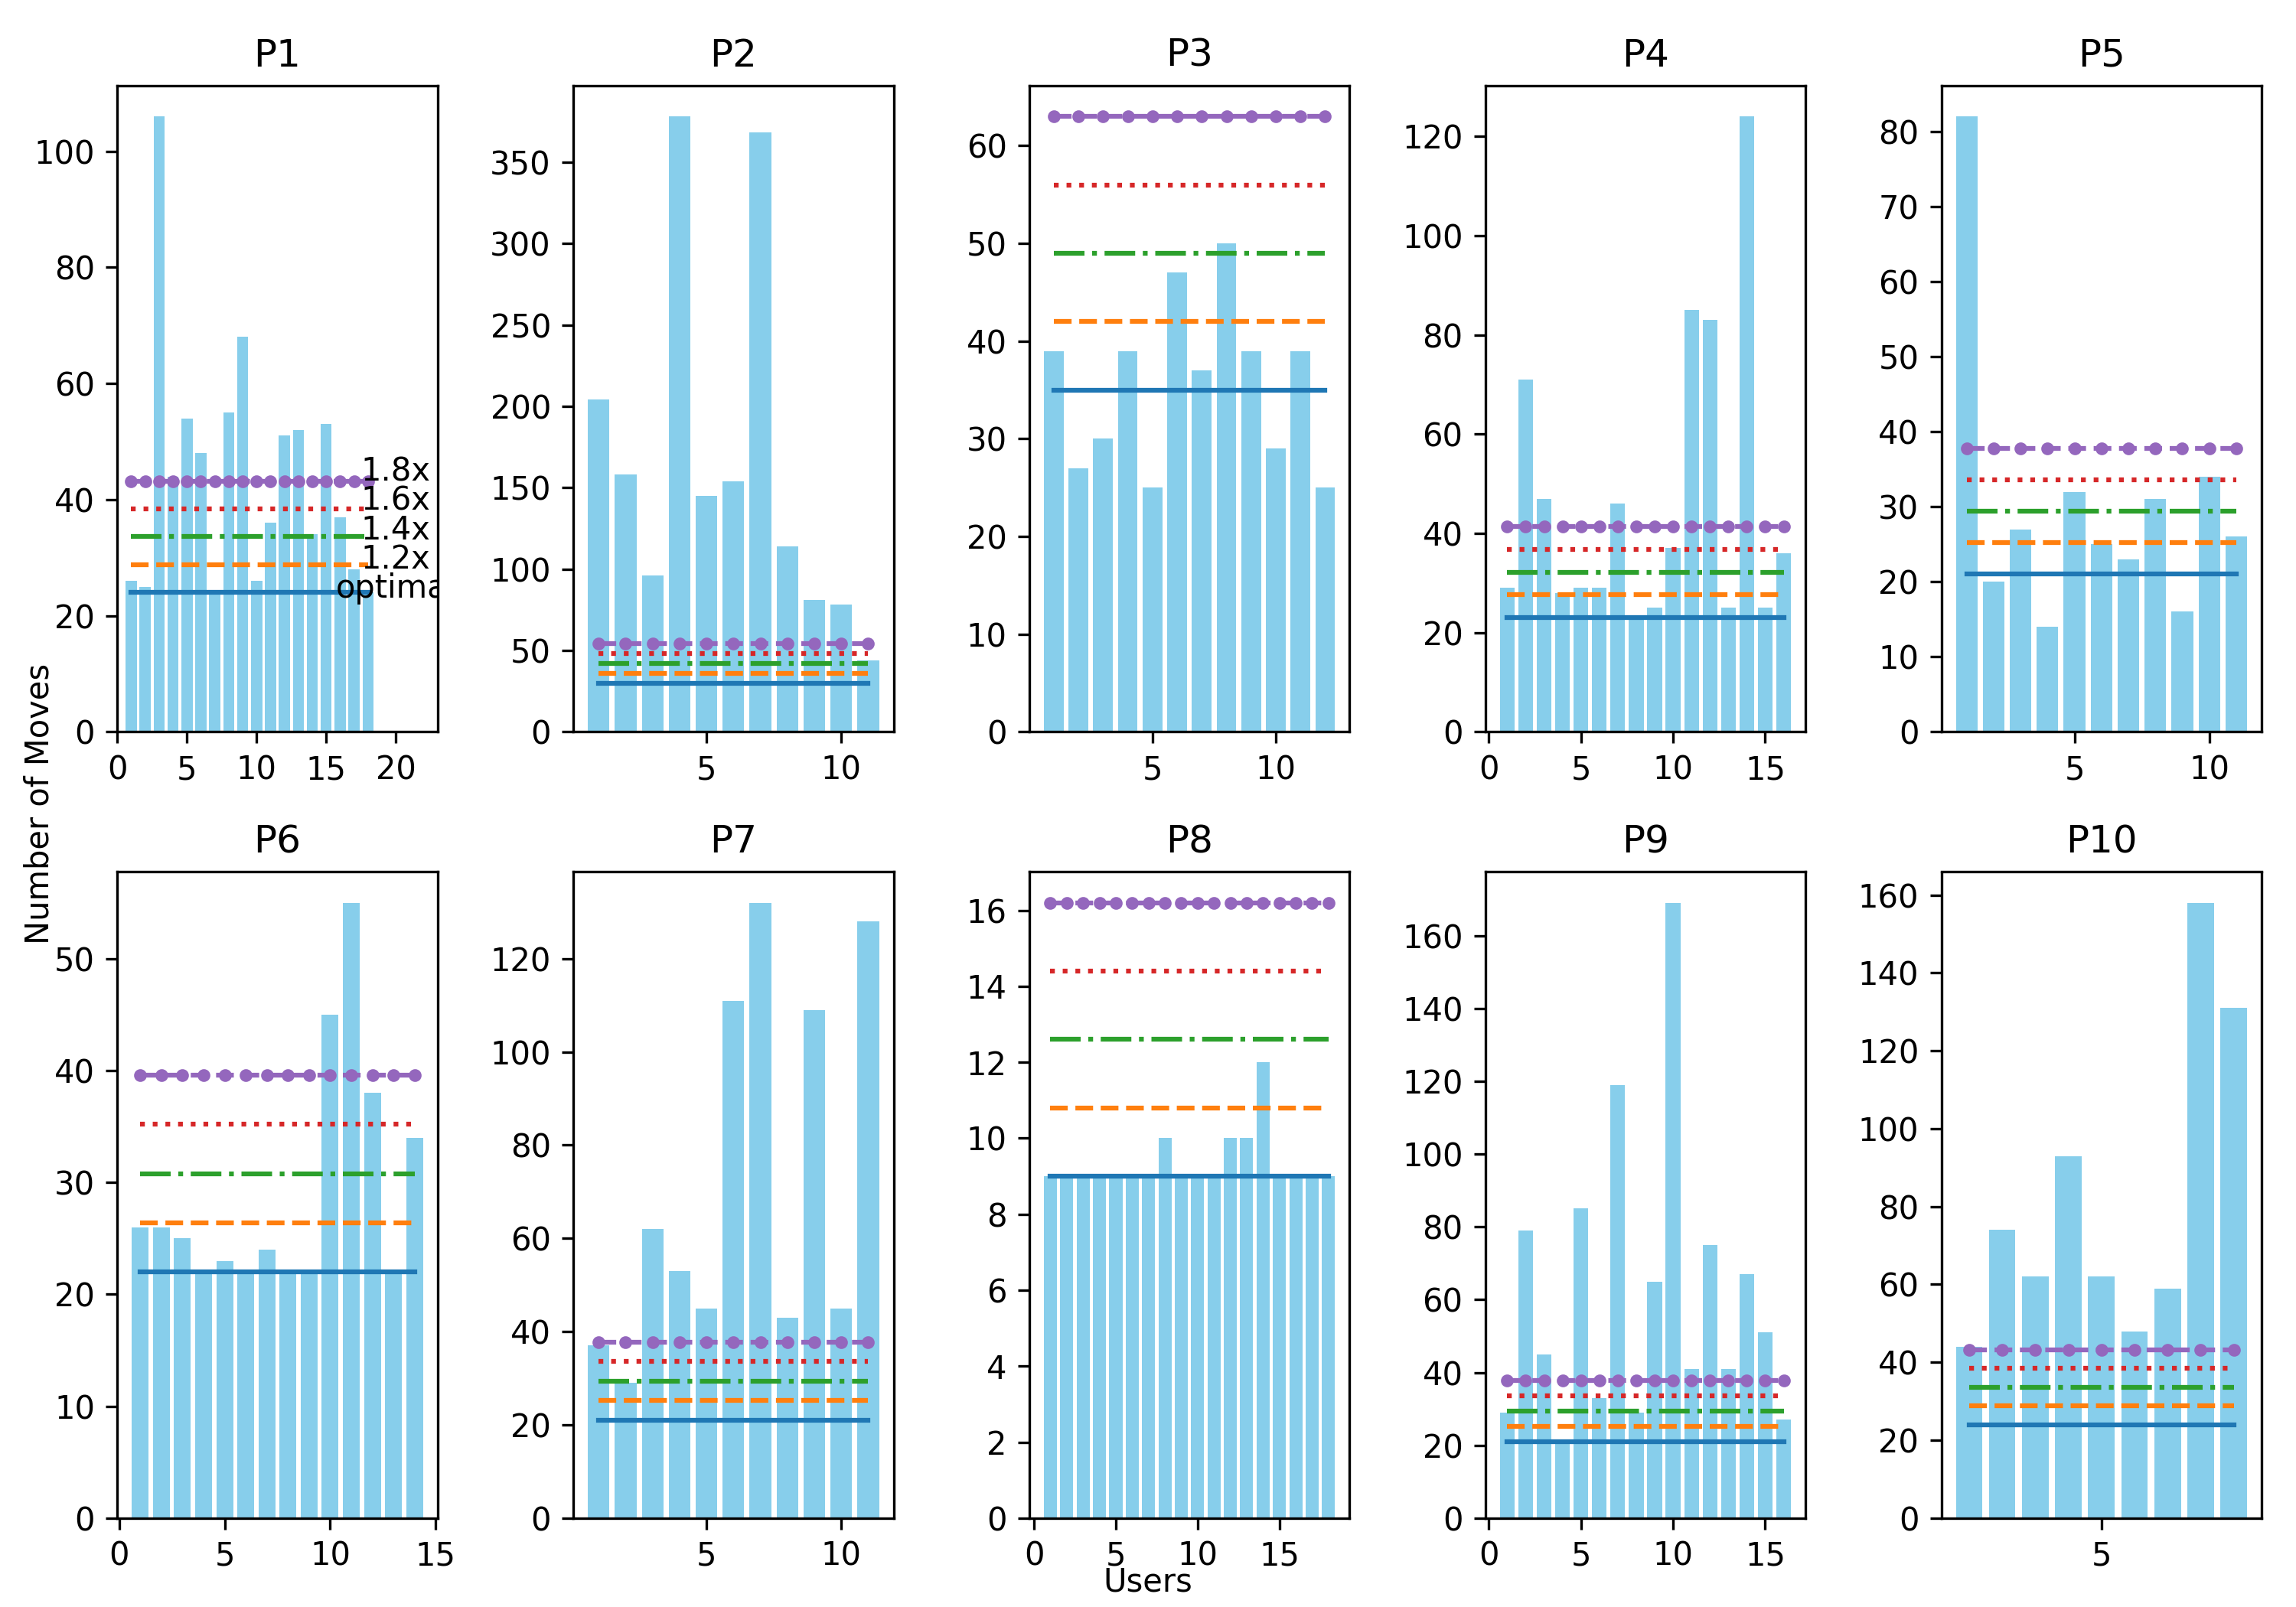
\includegraphics[width=\columnwidth]{img/difficulty.png}
  \caption{Number of moves in the users' solution compared to the optimal number of moves, and 1.2x, 1.4x, 1.6x, 1.8x the optimal number of moves for puzzles P1 through P10}
  \label{fig:difficuly}
\end{figure}

For each puzzle, we sorted users' solutions by the number of moves in the ascending order and split them into three groups (fast, medium, slow). We ensured that the three groups for each puzzle contained approximately equal number of users. Table \ref{tab:solvergroups} summarizes the findings. There were 46 users in the Fast group, 42 in the Medium and 48 in the Slow group. Mean refers to the mean number of moves in a solution produced by users who solved a specific puzzle. Forbidden moves refers to the number of times, the users who solved a specific puzzle moved the forbidden vehicle. Here, we consider the complete solution (i.e., moves from the initial state to the goal state).

\begin{table}[ht]
\begin{tabular}{|l|l|l|l|l|l|l|}
\hline
\multicolumn{1}{|c|}{\multirow{2}{*}{PID}} &
  \multicolumn{2}{c|}{Fast (46)} &
  \multicolumn{2}{c|}{Medium (42)} &
  \multicolumn{2}{c|}{Slow (48)} \\ \cline{2-7} 
\multicolumn{1}{|c|}{} &
  \multicolumn{1}{c|}{Mean} &
  \multicolumn{1}{c|}{\begin{tabular}[c]{@{}c@{}}Forbidden\\ Moves\end{tabular}} &
  \multicolumn{1}{c|}{Mean} &
  \multicolumn{1}{c|}{\begin{tabular}[c]{@{}c@{}}Forbidden\\ Moves\end{tabular}} &
  \multicolumn{1}{c|}{Mean} &
  \multicolumn{1}{c|}{\begin{tabular}[c]{@{}c@{}}Forbidden\\ Moves\end{tabular}} \\ \hline
P1  & 25.5 & 0  & 41.7  & 0  & 64.7  & 0  \\ 
P2  & 74.7 & 4  & 137.7 & 16 & 277   & 28 \\ 
P3  & 26.5 & 8  & 36.2  & 9  & 43.7  & 6  \\ 
P4  & 25.2 & 1  & 32    & 4  & 76    & 28 \\ 
P5  & 18.3 & 3  & 26    & 2  & 44.75 & 13 \\ 
P6  & 22   & 0  & 24.5  & 0  & 39.6  & 0  \\ 
P7  & 38.5 & 5  & 53.3  & 16 & 120   & 37 \\ 
P8  & 9    & 0  & 9     & 0  & 10    & 0  \\ 
P9  & 27.8 & 8  & 48.6  & 12 & 99    & 28 \\ 
P10 & 50.3 & 11 & 66    & 14 & 127.3 & 46 \\ \hline
\end{tabular}
\caption{Human solvers grouped by the mean number of moves and the corresponding forbidden moves}
\label{tab:solvergroups}
\end{table}

We can see that the longer the users' solutions are the more they will be moving the forbidden vehicle. Is this relationship statistically significant? We first perform the normality test between the two variables: number of moves and the number of times the forbidden car was moved. We used the Shapiro-Wilks test for the two distributions with $H_0:$ the distribution is normally distributed, and $H_A:$ the distribution is not normally distributed. Given $\alpha=0.05$, Shapiro-Wilks test gives that the p-value $<0.05$ for both forbidden vehicle moves and the number of moves. Thus we reject $H_0$ for both distributions.

To test the relationship between the number of moves and the forbidden vehicle moves, we define the null and alternative hypotheses as follows. Since we showed that there is evidence that the distributions are not normally distributed, we use the non-parametric test, Spearman's Rank Correlation to test the strength of relationship. Let $\rho_s$ be the Spearman's population correlation coefficient:
\begin{itemize}
\item $H_0: \rho_s=0$, there is no correlation between the two variables
\item $H_A: \rho_s\neq0$, there is a correlation between the two variables
\end{itemize}
Given $\alpha=0.05$, Spearman's rank correlation coefficient is $\rho_s=0.52$ and p-value $<0.05$. Thus we reject the null hypothesis.

We now describe the behavior features we extract from a partial solution.
\begin{description}
\item[\texttt{len}:] number of moves in the partial solution
\item[\texttt{len-opt}:] difference of the number of moves in the user's partial solution and the number of steps in the safe optimal solution produced by an automated planner
\item[\texttt{undos}:] number of 1-step undo in the user's partial solution
\item[\texttt{forbidden}:] number of times the forbidden vehicle is moved
\item[\texttt{first}:] number of moves until the forbidden vehicle was moved for the first time
\item[\texttt{prop}:] number of moves until the forbidden vehicle was moved for the first time divided by the number of moves in the safe, optimal solution
\item[\texttt{moved}:] number of vehicles moved in the partial solution
\end{description}

\subsection*{Learning Methods}
We ask three learning questions:
\begin{itemize}
\item Can we predict whether or not the user will move the forbidden car one step before it actually happens?
\item Can we predict whether or not the user will move the forbidden car two steps before it actually happens?
\item Can we predict whether or not the user will move the forbidden car there steps before it actually happens?
\end{itemize}

In order to answer these three questions, we first partition the data set into training (70\%) and test (30\%) sets. Each user solution is filtered to only include the moves until one step, two steps and three steps before the forbidden car was moved for the first time. We then filter the features to remove features that are obvious indicators of forbidden car movements, specifically first, prop and forbidden. We use the remaining features to train five classifiers to respond to each learning question with 10-fold cross validation. In this work, we explore a number of classifier learning methods: the decision tree, random forest, K-nearest neighbor, Logistic Regression and Naive Bayes. The classifiers are used in the supervised learning mode. We summarize the parameters used in each learning method below:
\begin{itemize}
\item \textit{Decision Tree:} We use the J48 classifier available on the WEKA platform \cite{hall09}. This classifier implements the C4.5 algorithm \cite{quinlan1993c45}. The decision tree classifier is tuned to user pruning confidence=0.25 and the minimum number of instance per leaf=2.
\item \textit{Random Forest:} This classifier is tuned to use bagging with 100 iterations and a base learner. These configuration parameters are available on the WEKA platform. 
\item \textit{k Nearest Neighbor:} We use this classifier with a Euclidean distance metric, considering the value $k=1$
\item \textit{Logistic Regression:} This classifier is tuned for ridge parameter $= 1.0E-8$.
\item \textit{Naive Bayes:} This classifier is tuned with the supervised discretization=True.
\end{itemize}

\subsection*{Results}
We then use each learned model on the test data set to predict the class for each user, i.e, whether the user be intervened or not given his partial solution. Table \ref{tab:accuracy} summarizes the precision, recall and F-measures for the three soft intervention models.
It can be seen that the Logistic Regression classifier performs best with high precision/recall compared to other classifiers when predicting soft intervention 1 or 2 steps early. The Logistic Regression classifier also predicts intervention 3 steps early with high recall albeit with slightly lower precision. As the prediction window expands, the precision of the decision tree classifier improves. However, the recall and F measures drop when predicting intervention 3 steps early. The Naive Bayes classifier reported the lowest precision compared to all other classifiers for all three intervention windows. It is interesting to note that the Random Forest classifier performs better than the Decision Tree when the intervention window is 1 and 3 steps. The accuracy drops for the Random Forest when the prediction window is 2.

\begin{table}[htb]
\begin{tabular}{|l|l|l|l|}
\hline
Q1 &
  \multicolumn{3}{l|}{\begin{tabular}[c]{@{}l@{}}Predict whether the user will be moving the forbidden car one\\ step before the move actually happens\end{tabular}} \\ \hline
\textbf{Classifier} &
  \textbf{Precision} &
  \textbf{Recall} &
  \textbf{F1} \\ \hline
Decision Tree       & 0.7  & 0.9  & 0.79 \\ 
Random Forest       & 0.76 & 0.9  & 0.83 \\ 
k Nearest Neighbor  & 0.89 & 0.76 & 0.82 \\
Logistic Regression & 0.91 & 0.95 & 0.93 \\ 
Naive Bayes         & 0.73 & 0.9  & 0.81 \\\hline
Q2 &
  \multicolumn{3}{l|}{\begin{tabular}[c]{@{}l@{}}Predict whether the user  will be moving the forbidden car two\\ steps before the move actually happens\end{tabular}} \\ \hline
Decision Tree       & 0.8  & 0.95 & 0.87 \\
Random Forest       & 0.75 & 0.86 & 0.8  \\ 
k Nearest Neighbor  & 0.86 & 0.86 & 0.86 \\ 
Logistic Regression & 0.87 & 1    & 0.93 \\
Naive Bayes         & 0.74 & 0.86 & 0.83 \\ \hline
Q3 &
  \multicolumn{3}{l|}{\begin{tabular}[c]{@{}l@{}}Predict whether the user  will be moving the forbidden car three\\ steps before the move actually happens\end{tabular}} \\ \hline
Decision Tree       & 0.89 & 0.81 & 0.85 \\ 
Random Forest       & 0.86 & 0.9  & 0.88 \\
k Nearest Neighbor  & 0.95 & 0.9  & 0.93 \\ 
Logistic Regression & 0.91 & 0.95 & 0.93 \\ 
Naive Bayes         & 0.68 & 0.9  & 0.78 \\ \hline
\end{tabular}
\caption{Precision, Recall and F-measure for the prediction accuracy for the three soft intervention learned models.}
\label{tab:accuracy}
\end{table}

\section*{Supporting Human Users with Soft Intervention}
We extend our soft intervention model to help human users complete cognitively engaging tasks by providing helpful hints. In the context of the Rush Hour puzzle solving task, a hint is a piece of information about the Rush Hour search problem. Hints are a special type of answer because they do not directly provide the complete solution to the problem (e.g., remaining moves to solve the Rush Hour puzzle). Our design of helpful hints allows the user to carefully probe the search space of the Rush Hour puzzle while avoiding the undesirable state. Hints are specially useful in situations where the human user wishes to retain some autonomy over the system he is interacting with (e.g., intelligent tutoring systems).
Formally, a hint is a function of the state space of the search problem. We represent the Rush Hour search problem as the planning task $\Pi_{agent}$ and the solution to which is a plan $\pi_{agent}$.
\begin{definition}
Given a partial user solution $\pi^\prime _{user}$, the initial state $I$, the user's goal $G_x$, and the undesirable state to avoid is $G_y$, we define the current state $s = \Delta (I,\pi^\prime _{user})$. Then, a hint is a function defined as: $\mathcal{H}(s,\lbrace G_x,G_y\rbrace) \rightarrow \Psi[\pi_{agent}]$, where $\Psi[\pi_{agent}]$ refers to some information about the solution plan $\pi_{agent}$.
\end{definition}
We conducted a human subject experiment to evaluate five hint types.
\begin{itemize}
\item Number of remaining moves, if $\Pi_{agent}$ is solved optimally, optimized for the number of moves.
\item Next move, if $\Pi_{agent}$ is solved optimally, optimized for the number of moves
\item The list of vehicles that must be moved to solve $\Pi_{agent}$
\item Restart game (i.e, restore $s$ back to $I$)
\item Ignore hint. Two successive choices of this option disables the hints.
\end{itemize}

For this study, we recruited 140 subjects from a graduate and undergraduate university student population. The participants were not compensated for their time. The sample comprised of college undergraduate and graduate students in Computer Science, Microbiology, Chemistry, Business majors. After obtaining informed consent, the participants were directed to the Web URL, which hosted the Rush Hour simulator software. In this study, we added three new functional features to the simulator, namely: an automated planner to probe the search space, a landmark computation component to support hint generation, and the soft intervention learned model.

Each participant was assigned to solve one Rush Hour puzzle randomly selected from a set of thirteen. We did not place any time restriction for the puzzle solving task. Participants were randomly assigned to two groups; one group was asked to watch a 44 second video tutorial on how the Rush Hour puzzle can be solved by avoiding the forbidden vehicle. This group was only allowed to start the puzzle after watching the video. The other group did not watch the video. Instead they were allowed to immediately start the puzzle. Additionally, all participants had the option to use an online tutorial (available on the simulator itself) on how to play the Rush Hour puzzle. Each of the thirteen puzzles contained one forbidden vehicle. Participants were informed that one of the vehicles on the game board is forbidden and the puzzle must be solved without moving the forbidden vehicle. In this phase, the simulator produced an alert message when the soft intervention learned model predicted that, based on the user's partial solution, the user will be moving the forbidden vehicle 1 move later. The alert message displayed the five hints (see Figure \ref{fig:help}) and the user is asked to select one. Based on the choice, a second alert message is shown, which contains the information $\Psi[\pi_{agent}]$. Once the puzzle solving task was completed, the participants were asked to complete a short demographic survey and rate the helpfulness of each hint type in avoiding the forbidden vehicle. Figure \ref{fig:phase2} illustrates the activity sequence of the experiment.

\begin{figure}[!htb]
  \centering
  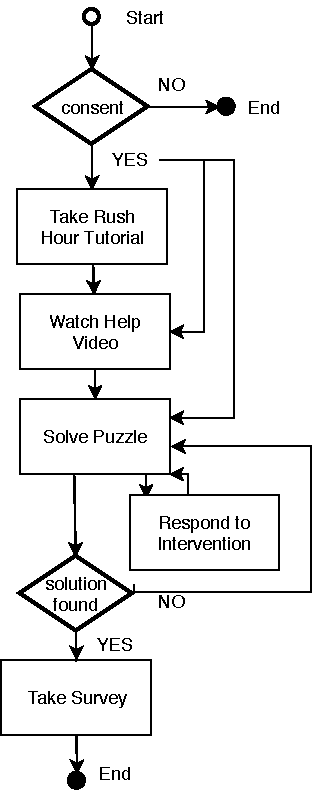
\includegraphics[height=0.6\columnwidth]{img/phase2.pdf}
  \caption{Activity sequence for evaluating hints during intervention for the Rush Hour human subject experiment}
  \label{fig:phase2}
\end{figure}

\subsection*{The Planning Component}
Two of the hints: number of remaining moves and next move, use the planning component. Our design of the planning component use the Fast Downward planner \cite{helmert2006} with the LM-cut heuristic (admissible) to find optimal plans, optimized for the number of moves. Given a partial user solution $\pi^\prime _{user}$, the initial state $I$, the user's goal $G_x$, and the undesirable state to avoid is $G_y$, we define the current state $s = \Delta (I,\pi^\prime _{user})$. Then, the planning component generates the planning task $\Pi_{agent} = \langle \mathcal{F}, \mathcal{A}, s, G \rangle$, where $\mathcal{F}$ is the propositions grounded with the objects $\mathcal{O}\setminus o_f$ where $o_f$ is the forbidden vehicle, $\mathcal{A}=A_d$ (i.e., actions that are not grounded with $o_f$), $s$ is the new initial state (i.e., state after executing the partial solution) and $G = G_x$ (i.e, target vehicle being at the exit).
The solution to $\Pi_{agent}$ is the plan $\pi_{agent}$, which is a sequence of actions $\lbrace a_1, a_2, \ldots, a_n\rbrace$, where $a_i \in \mathcal{A}$. Because we are using an admissible heuristic to find the plan, $\pi_{agent}$ is also the optimal plan to solve the puzzle from the current state $s$. When the user requests for the hint \textbf{number of remaining moves}, $\Psi[agent]=c(\pi_{agent})$, which refers to the cost of $\pi_{agent}$. Since we are assuming actions are of unit cost, this is equivalent to the number of actions in $\pi_{agent}$. This hint gives the user an indication of how many more moves the user needs to minimally make to solve the puzzle from the current state while avoiding the undesirable state. Similarly, when the user requests for the hint \textbf{next move}, $\Psi[agent]=a_1$, which is the first action in $\pi_{agent}$. This information tells the user the next action to execute if the user were to solve the puzzle with the minimum number of moves from the current state while avoiding the undesirable state.

The hint for the \textbf{list of vehicles that must be moved} requires us to find the landmarks for the planning task $\Pi_{agent}$. \textit{A landmark of a planning task are facts that must be true at some point during the execution of any solution plan} \cite{hoffman2004lm}. By this definition, the initial and the goal facts are trivially landmarks. We use the Ordered Landmark algorithm \shortcite{hoffman2004lm} to find landmarks in the planning task $\Pi_{agent}$. This algorithm uses a data structure called the Landmark Generation Graph (LGG) to find the landmarks and the greedy necessary orders between them. Nodes in LGG are the landmark propositions and the edges are the greedy-necessary orders. Starting from the goal (the first landmark candidates), the algorithm uses the back-chaining process to find the earliest actions that can be used to achieve each landmark. Here, early means a greedy approximation of reachability from the initial state. The landmark achievers are actions in $\mathcal{A}$. The landmark achievers are grounded with the objects that must be moved to solve the puzzle from the current state.

The two other hints \textbf{Restart} and \textbf{Ignore} are the last-resort kind of help. The restart game hint simply reverts the game state $s$ back to the initial state $I$ and allows the user to start from the beginning. In the experiment setup, we did not enforce any limits on the number of times a participant can restart a game. The ignore hint allows the user to continue the puzzle solving task. This does not modify the current game state. However, in the experiment setup we enforced a condition that if the participant selects the ignore option twice in a row, the intervention help system will permanently deactivate.

\subsection*{The Learning Component}
We use the Logistic Regression classifier learned from human solvers' solutions in the previous study to predict intervention in this experiment. Our learned models operate within three intervention intervals, where the user is intervened either one step before, two steps before or three steps before the forbidden vehicle is moved. For this experiment, we used the Logistic Regression classifier trained to intervene one step before the undesirable state. This classifier had the highest precision, recall and F measures compared to all other classifiers we experimented with.

Given a partial user solution $\pi^\prime _{user}$, and the initial state $I$, we define the current state $s = \Delta (I,\pi^\prime _{user})$. We then compute the feature values corresponding to the current game state ($s$) and also the feature values corresponding to the partial solution $\pi^\prime _{user}$. Then the feature vector combining both game state and partial solution features are provided as input to the classifier and a decision is obtained whether to intervene or not. If an intervention occurs the user is shown a set of hints. If not the user continues to solve the puzzle. This cycle continues for each new move the user makes unless the user instructs the system to stop intervention by choosing the Ignore Hint option.

%results
\subsection*{The Human Subject Experiment}
\subsubsection*{Experimental Design}
Our second human subject experiment evaluates how human solvers use the helpful hints during the Rush Hour puzzle solving task. As shown in Table \ref{tab:puzzles} (right), we created thirteen unique Rush Hour puzzles. We used ten puzzles (P1 through P10) from the previous study and added three new puzzles so that each puzzle type (A, B, C) had approximately the same number of puzzles. For this study, we recruited subjects from a graduate and undergraduate university student population. The participants were not compensated for their time. After obtaining informed consent, the participants were directed to the Web URL, which hosted the Rush Hour simulator software. In this experiment, the simulator software lets the user solve a puzzle but offers helpful hints upon recognizing the user may move the forbidden vehicle 1 step ahead into the future.

Before starting the puzzle solving task, the participants were randomly assigned to two groups. One group were shown a 44 second video of a Rush Hour puzzle solving task. The video showed a solution, which did not move the forbidden vehicle. Participants in this group were only allowed to continue on to the puzzle solving task after watching the video. Figure\ref{fig:video} illustrates the video screen. The other group did not see the video and was directed to start the puzzle solving task immediately. Each participant was assigned to solve one Rush Hour puzzle randomly selected from the set of thirteen. We did not place any time restriction for the puzzle solving task. All participants had the option to use an online tutorial (available on the simulator itself) on how to play the Rush Hour puzzle. All thirteen puzzles contained a forbidden vehicle. Participants were informed that one of the vehicles on the game board is forbidden and the puzzle must be solved without moving the forbidden vehicle. 

\begin{figure}[!htb]
  \centering
  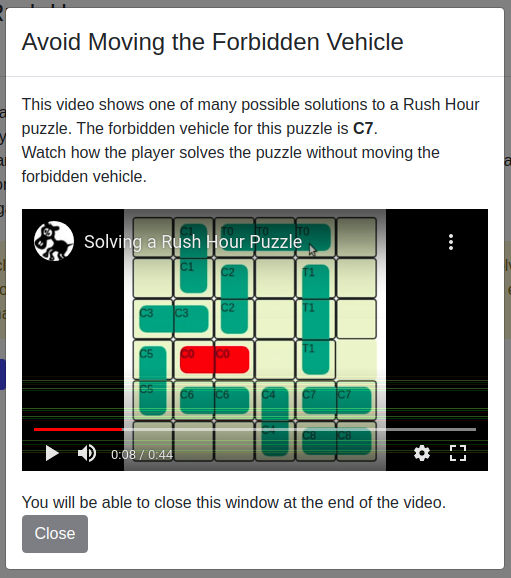
\includegraphics[width=0.6\columnwidth, keepaspectratio=true]{img/help.png}
  \caption{Help video screen}
  \label{fig:video}
\end{figure}

During the puzzle solving task when the decision to intervene is made, the participant sees pop-up message shown in Figure \ref{fig:help}, which offers four hints and the ignore option. Based on the choice the user makes, a response is displayed. In addition, if the user moves the forbidden vehicle the simulator displays an alert shown in Figure \ref{fig:badcar}. When this happens, the game engine automatically undoes the forbidden vehicle move. These functionalities are different from the previous experiment conditions where the participant did not get any visual cues during game play.
\begin{figure}[!htb]
  \centering
  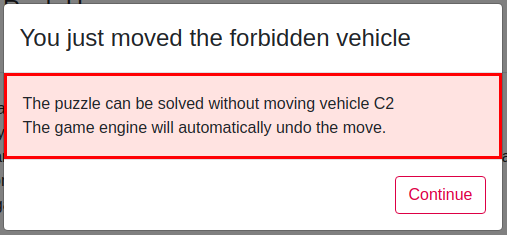
\includegraphics[width=0.5\columnwidth, keepaspectratio=true]{img/badcaralert.png}
  \caption{Forbidden vehicle move alert message}
  \label{fig:badcar}
\end{figure}
Once the puzzle solving task is completed, the participants are asked to complete a short survey to capture the demographics and also asks them to subjectively rate the helpfulness of each hint type on a 5-point Likert scale. 142 subjects participated the study. We removed records from seven participants from the analysis because they had quit the session mid-play, leaving 135 usable records. The sample comprised of college undergraduate and graduate students in Agriculture, Biology, Animal Sciences, Computer Science, Engineering, Horticulture, and Business majors. 131 of the 135 participants also completed the demographics survey.
